\documentclass{report}
\usepackage{graphicx} % Required for inserting images
\usepackage{alltt, fancyvrb, url}
\usepackage{graphicx}
\usepackage[utf8]{inputenc}
\usepackage{float}
\usepackage{hyperref}
\usepackage{amsmath}
\usepackage{amssymb}
\usepackage{amsfonts}
\usepackage{amsmath, bm, tabularray}
\usepackage[left=2.5cm, right=2.5cm, bottom=2.5cm]{geometry}
\title{Ingeria del Software}
\author{luca carabini}
\date{September 2023}

\begin{document}
\maketitle
\tableofcontents
\chapter{I protocolli di Internet}
    \section{Arcitettura}
        \begin{figure}[H]
            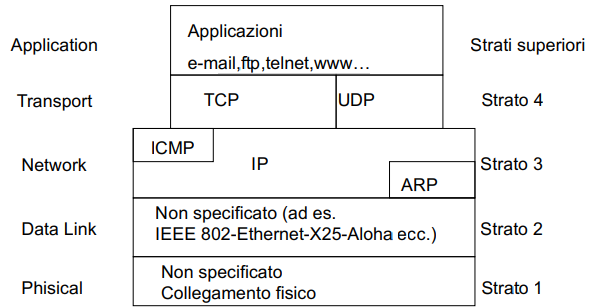
\includegraphics[width=0.9\textwidth]{1/Architettura.png}
        \end{figure}
    \section{Internet Protocol(IP)}
        È stato progettato per funzionare a \textbf{commutazione di pacchetto} in modoalità \textbf{connectionless}
        \\
        Si prende carico della trasmissione di datagrammi da sorgente a destinazione, attraverso reti eterogenei.
        \\
        Identifica host e router tramite indirizzi di lunghezza fissa, raggruppandoi in reti IP
        \\
        Frammenta e riassembla i datagrammi quando necessario
        \\
        Offre un servizio di tipo best effort, cioè non sono previsti meccanismi per:
        \begin{itemize}
            \item aumentare l'affidabilità del collegamento end-to-end
            \item eseguire il controllo di flusso e della sequenza
        \end{itemize}
        \subsection{La struttura degli indirizzi IP}
            La loro lunghezza è fissa e pari a 32 bit, che convenzionalmente sono scritti come sequenza di 4 numeri decimali che vanno da 0 a 255 separati da un punto.
            \\
            Il numero teorico massimo di indirizzi è $2^{32}$ (in realtà si riesce a sfruttare un numero molto inferiore)
            \\
            Sono assegnati dalla IANA (Internet Assigned Numbers Authority)
    \section{Formato del pacchetto}
         \begin{figure}[H]
            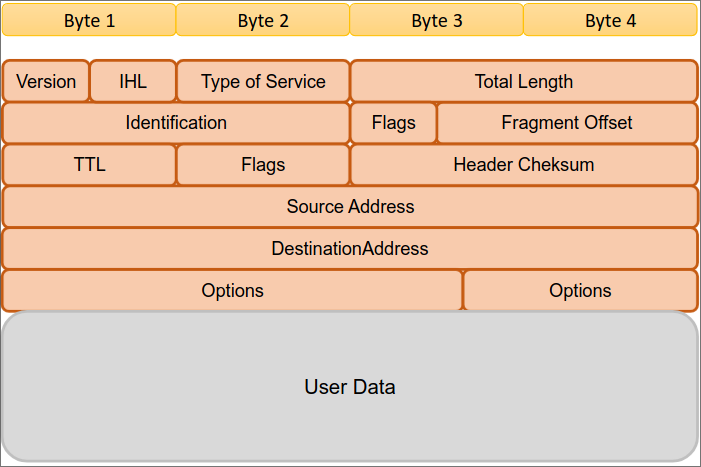
\includegraphics[width=0.9\textwidth]{1/PCI.png}
        \end{figure}
        \begin{itemize}
            \item \textbf{Verision} : indica il formato dell'intestazione
            \item \textbf{IHL} : lunghezza dell'intestazione, espressa in parole di 32 bit
            \item \textbf{Type of service} : indicazione sul tipo di servizio richiesto
            \item \textbf{Total length} : lunghezza totale del datagramma, misurata in bytes, la lunghezza massima è 65535 bytes (non è detto che tutte le implementazioni siano in grado di gestire questa dimensione)
            \item \textbf{Identification} : valore intero che identifica univocamente il datagramma, indic a quale datagramma appartiene un fragmento
            \item \textbf{Flag}: 
                \begin{itemize}
                    \item \textbf{bit 0} : sempre a zero
                    \item \textbf{bit 1} : don't fragment (DF), DF=0 si può fragmentare, DF=1 non si può fragmentare
                    \item \textbf{bit 2} : more fragment (MF), MF=0 ultimo fragmento, MF=0 frammento intermedio
                \end{itemize}
            \item Fragment offset : indica qual è la posizione di questo fragmento nel datagramma, come distanza in unità di 64 bit dall'inizio
            \item Time to live (TTL) : max numero di nodi attraversabili :
                \begin{itemize}
                    \item Il nodo sorgente attribuisce un valore maggiore di 0 a TTL (tipicamente TTL=64, al massimo 255)
                    \item Ogni nodo che attraversa il datagramma pone TTL=TTL-1
                    \item Il primo nodo che vede TTL=0 distrugge il datagramma
                \end{itemize}
            \item \textbf{Protocol} : indica a quale protocollo di livello superiore appartengono i dati del datagramma
            \item \textbf{Header checksum} : controllo di errore della sola intestazione, viene ricalcolato da ogni nodo attraverso dal datagramma.
            \item \textbf{Source and Destination Address} : indirizzi sorgente e destinazione
            \item \textbf{Padding} : bit privi di significato aggiunti per fare in modo che l'intestazione sia con certezza multipla di 32 bit
        \end{itemize}
        \subsection{Fragment ofset}
            Il datagramma IP viene virtualmente suddiviso in sotto-blocchi di 8 byte(64 bit).
            \\
            Per l'IP che trasmette, il primo blocco del dtatagramma è il numero 0, i blocchi successivi sono logicamente numerati sequenzialmente, il numero logico del primo blocco viene scritto ne Fragment offset del datagramma
            \subsubsection{Imlementazione}
                Un qualunque apparato di rete dotato di protocollo IP può frammentare un datagramma, tipicamente i nodi intermedi non riabbleblano, ma lo fa solamente il terminale ricevente.
                \\
                Un datagramma può essere frammentato a più riprese in nodi successivi (Frammentazioni multiple)
                \\
                La numeriazione tramite "offset" permentte di rinumerare facilmente frammenti di un frammento
                \begin{figure}[H]
                    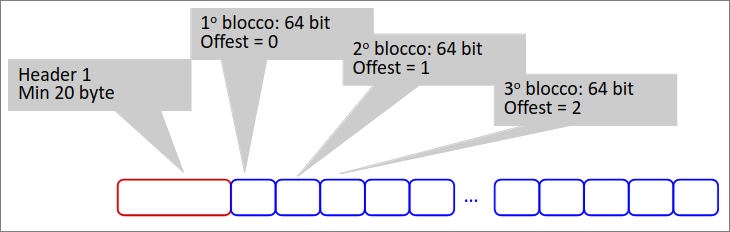
\includegraphics[width=0.9\textwidth]{1/offset.png}
                \end{figure}
            \subsubsection{Perchè la frammentazione}
                \begin{figure}[H]
                    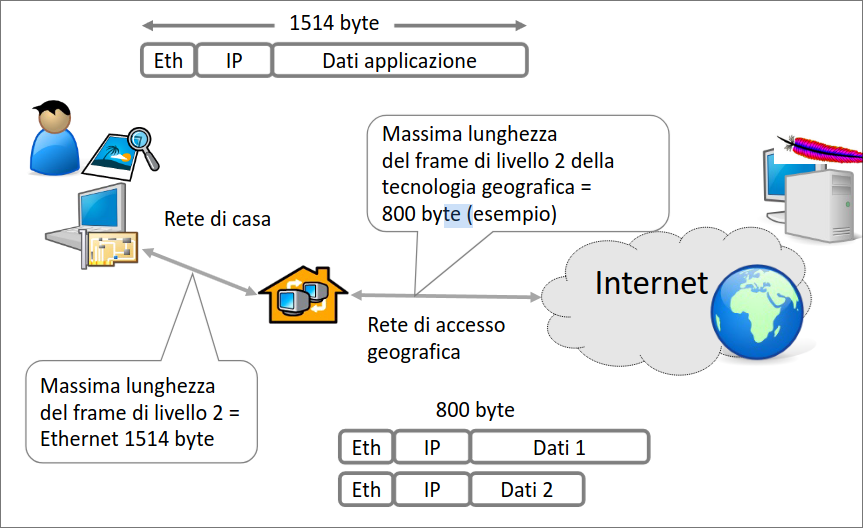
\includegraphics[width=0.9\textwidth]{1/seg.png}
                \end{figure}
            \subsubsection{Riassemblamento}
                \begin{figure}[H]
                    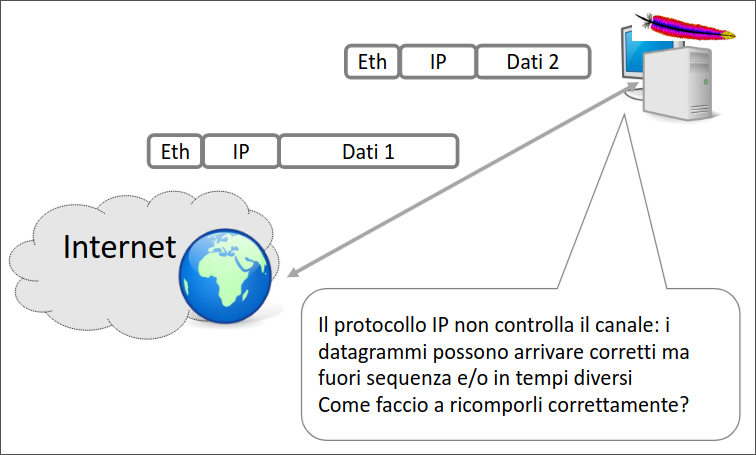
\includegraphics[width=0.9\textwidth]{1/rias.png}
                \end{figure}
            \subsubsection{Calcolo dell'offset}
                \begin{figure}[H]
                    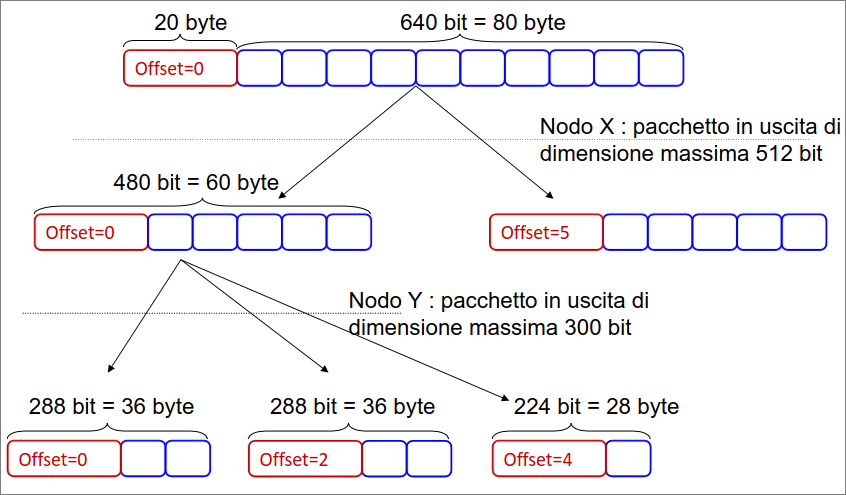
\includegraphics[width=0.9\textwidth]{1/calc.png}
                \end{figure}
    \chapter{Instradamento IP}
        La rete internet  una rete a commutazione di pacchetto, In generale esistono più modi per raggiungere una destinazione da una certa sorgente 
        \section{Come funziona Internet}
            Internet è una grande "rete di reti"
            \\
            La componente principale è la\textbf{ network IP}; ogni nettwork IP è una sorta di isola, e contiene calcolatori che fungono da nodi nella rete detti \textbf{host}.
            \\
            Le isole sono connesse da apparati che svolgono la funzione di "ponte", si tatta di calcolatori specializzati detti \textbf{router} o \textbf{gateway}.
        \section{Internet: rete di reti}
             \begin{figure}[H]
                    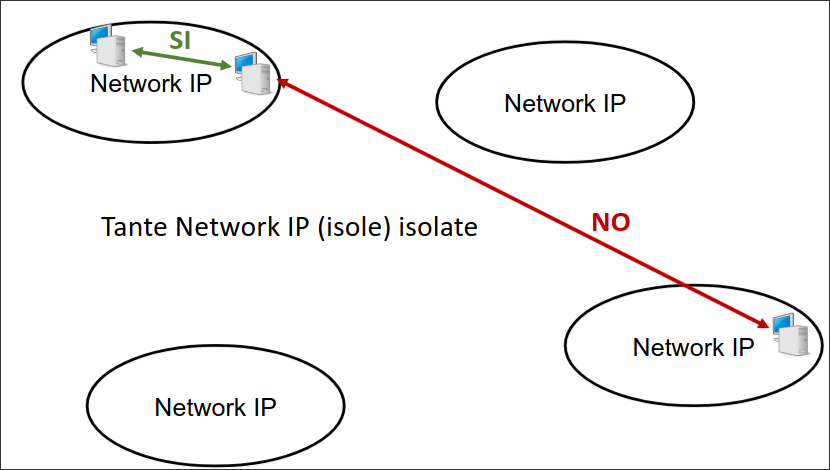
\includegraphics[width=0.9\textwidth]{1/rdr.png}
                \end{figure}
            \section{La tecnologia}
                Ogni network IP può essere implementata con una \textbf{tecnologia specifica}.
                \\
                Ad esempio:
                \begin{itemize}
                    \item Wi-Fi : Network realizzata con tecnologia wireless in area locale.
                    \item ADSL : Network realizzata con tecnologia a media distanza via cavo  tramite infrastruttura di uno specifico fornitore di servizio pubblico
                    \item Ethernet : Network realizzata con tecnologia a breve distanza via cavo privata in area locae
                    \item GPRS/EDGE/LTE :  Network realizzata con tecnologia radio a media distanza tramite infrastruttura di uno specifico fornitore di servizio pubblico
                \end{itemize}
            \section{La network IP}
                I calcolatori di una network IP sono connessi dalla medesima infrastruttura di rete fisica (livelli 1 e 2)
                \\ 
                Tutti gli host di una medesima nettwork IP sono in grado di parlare tra loro grazie alla tecnologia con cui essa viene implementata ( senza l'utilizzo di router o gateway)
                %TODO es terminale 
            \section{Rete logica e fisica}
                \textbf{Rete ogica} la network IP a cui un Host appartiene logicamente.
                \\
                \textbf{rete fisica} la rete (tipicamente LAN) a cui un Host è effetivamente connesso, normalmente ha capacità di instradamento e può avere indirizzi locali (es. indirizzi MAC)
                \\
                L'architettura a strati nasconde gli indirizzi fisici e consente alle applicazioni di lavolare solo con indirizzi IP.
            \section{Interconnettere le isole}
                Per far parlare tra di loro le isole (network IP) è necessario che:
                \begin{itemize}
                    \item Vi siano dei collegamenti fra le isole stesse, spesso realizzati con tecnologie diverse da quelle dell'isola.
                    \item Vi siano degli apparati che permettono di usare questi collegamenti nel modo opportuno
                    \item Sia possibile scegliere il giusto collegamento verso l'isola che si vuole ragiungere.
                \end{itemize}
                \subsection{I router}
                     \begin{figure}[H]
                    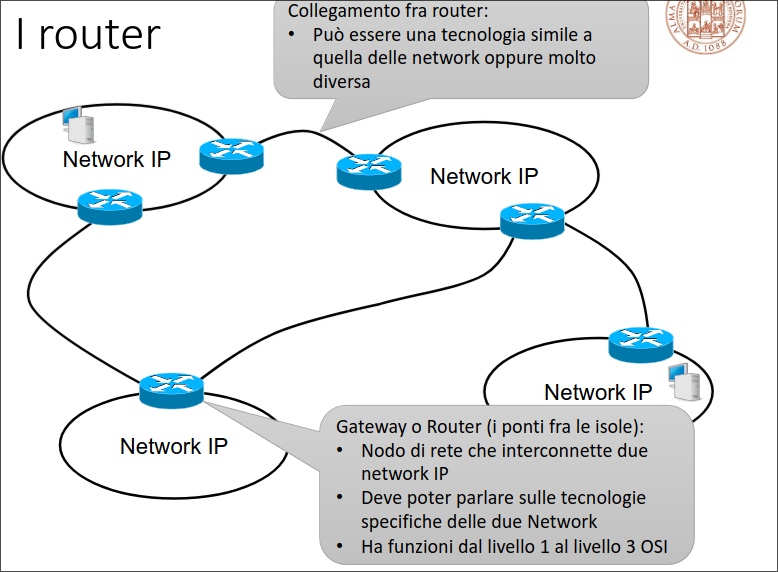
\includegraphics[width=0.9\textwidth]{1/router.png}
                \end{figure} \begin{figure}[H]
                    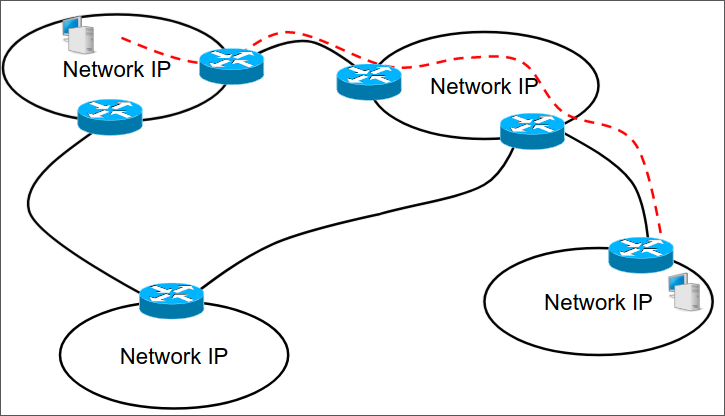
\includegraphics[width=0.9\textwidth]{1/router2.png}
                \end{figure}
                \subsection{Cosa fa IP}
                    La tecnologia IP è agnostica rispetto alla tecnologia con cui sono realizzate le network, quindi può lavorare indifferentemente su diverse tecnologie.
                    \\
                    L'obiettivo di IP è quello di rendere possibile il dialogo fra le network a prescindere dalla loro implementazione e localizzazione-
                \subsection{Ho un pacchetto da trasmettere, deve andare sulla mia network oppure devo usare un ponte?}
                    Ogni nodo di Internet ha una base dati di destinazioni possibili, quindi quando deve inviare un datatgramma:
                    \begin{itemize}
                        \item Parte dall'idirizzo IP destinazione
                        \item Legge la base dati 
                        \item Decide quale azione intraprendere
                    \end{itemize}
                    La tcnologia della propria network può essere utilizzata, per raggiungere la destinazione finale, o per raggiungere il primo ponte da attraversare
                    \begin{figure}[H]
                        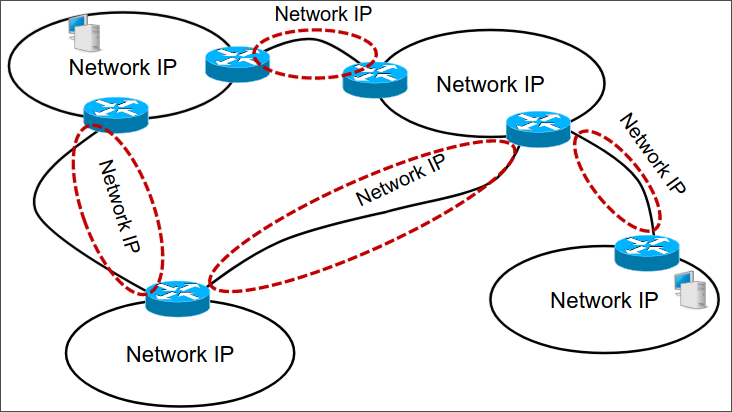
\includegraphics[width=0.9\textwidth]{1/ip.png}
                    \end{figure} 
                    \begin{figure}[H]
                        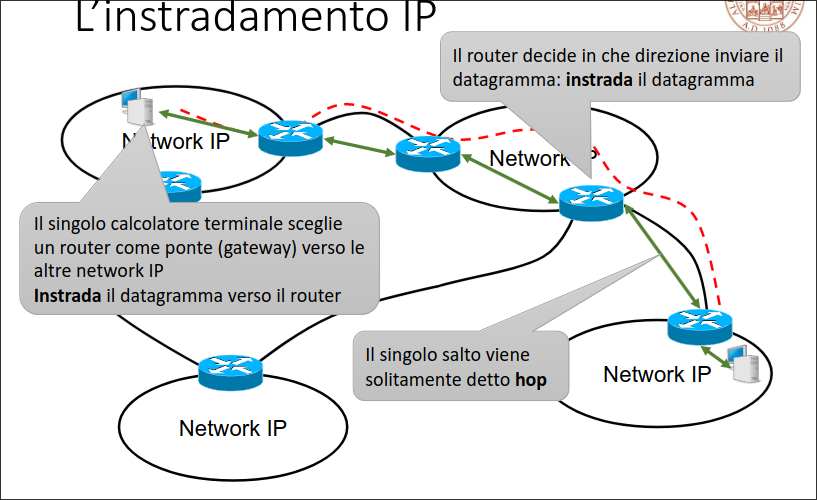
\includegraphics[width=0.9\textwidth]{1/ip2.png}
                    \end{figure}
            \section{Semantica dell'idirizzo IP}
                L'indirizzo IP è logicamente suddiviso in due parti:
                \begin{itemize}
                    \item \textbf{Network ID (Net ID)} : è il prefisso che identifica la Network IP a cui appartiene l'indirizzo, quindi tutti gli indiriizi di una medesima Network IP hanno lo stesso Net ID, e occupa la parte sinistra dell'indirizzo.
                    \item \textbf{Host ID} : Identifica l'Host (l' interfaccia) vero e proprio di una certa Network, occupa la parte destra dell'indirizzo
                \end{itemize}
                \subsection{Reti IP private(RFC 1918)}
                    Alcuni gruppi di indirizzi sono riservati a reti IP private, non sono raggiungibili dalla rete pubblica.
                    \\
                    I router di Internet non instradano datagrammi destinati a tali indirizzi.
                    \\
                    Possono essere riutilizzati in reti isolate.
                    \\
                     \begin{figure}[H]
                    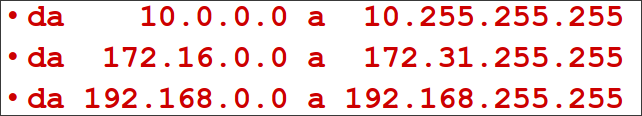
\includegraphics[width=0.9\textwidth]{1/retiP.png}
                \end{figure}
                \subsection{Come si distingue net-ID da host-ID}
                    Si usa la netmask, al numero IP viene associata una mascera di 32 bit, i bit a 1 nella netmask identificano i bit dell'indirizzo IP che fanno parte del net-ID
            \section{Instradamento diretto e indiretto}
                \subsection{Instradamento diretto}
                    Nel \textbf{Direct delivery} l'IP sorgente e l'IP destinazzione sono sulla stessa network, e l'host sorgente spedisce il datagramma direttamente al destinatario
                \subsection{Instradamento diretto}
                    Nell' \textbf{Indirect delivery} l'IP sorgente e L'IP destinatario, non sono sulla stessa network, l'host sorgente invia il datagramma ad un router intermedio
                \subsection{Routing}
                    Il routing è la scelta del percorso su cui inviare i dati, i router formano una struttura interconnessa e cooperante, i datagrammi passano dall'uno all'altro finchè non raggiungono quello che può consegnarli direttamente al destinatario 
            \section{Relazione indirizzi fisici - IP}
                Il software di basso livello nasconde gli indirizzi fisici e consente di lavorare ai livelli superiori con gli indirizzi IP.
                \\
                Gli Host comunicano attraverso una rete fisica (es. LAN) quindi devono conoscere reciprocamente gli indirizzi fisici.
                \\
                L'host A vuole mandare datagrammi a B, che si trova sulla stessa rete fisica e di cui conosce solo l'indirizzo IP.(come ricava l'indirizzo fisico?)
                \subsection{Adfress Resolution Protocol (ARP)}
                    \begin{figure}[H]
                        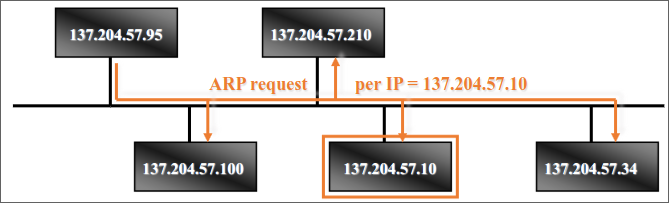
\includegraphics[width=0.9\textwidth]{1/arp.png}
                    \end{figure}
                    Il nodo sorgente invia una trama broadcast (\textbf{ARP request}) contenente l'indirizzo IP del nodo destinazione. 
                    \\
                    Tutte le stazioni della rete locale leggono la trama broadcast
                     \begin{figure}[H]
                        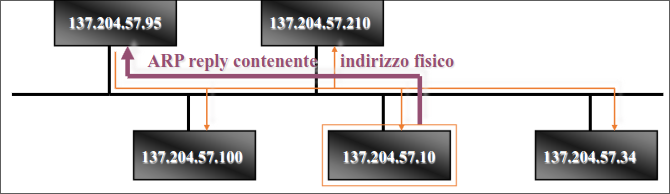
\includegraphics[width=0.9\textwidth]{1/arp2.png}
                    \end{figure}
                    Il destinatario risponde al mittente, inviando un \textbf{ARP reply} che contiene il proprio indirizzo fisico, l'host sorgente ora è in grado di associare l'appropriato indirizzo fisico all'IP destinazione.
                    \\
                    Ogni host mantiene una tabella (\textbf{cache ARP} con le corrispondenze fra indirizzi logici e fisici.
                    %TODO comando arp -a
            \section{Da mittente a destinatario} 
                C'è sempre un aconsegna diretta, può non esserci una consegna indiretta, e possono esserci una o più consegne indirette.
            \section{Tabella di instradamento IP}
                Base dati in forma di tabella:
                \begin{itemize}
                    \item \textbf{Righe (route)} : Insieme di informazioni relative alla singola informazione di instradamento. I suoi tipic campi sono:
                    \begin{itemize}
                        \item Destinazione(D): numero IP valido (può essere indirizzo di Host o di network)
                        \item Netmask(N) : mascera di rete valida (identifica il net-ID)
                        \item Gateway(G) : numero IP a cui consegnare il datagramma (indica il tipo di consegna da effetuare)
                        \item Interfaccia di rete(IF) : interfaccia di rete utilizzata per la consegna del datagramm (seleziona il dospositivo hardware da utilizzare per l'invio del datagramma)
                        \item Metrica(M) : specifica il "costo" di quel particolare route (Possono esistere più route verso una medesima destinazione).
                    \end{itemize}
                    \item \textbf{Colonne (campi)} : Informazioni del medesim tipo relative a diverse opzioni di instradamento.
                \end{itemize} 
                \begin{figure}[H]
                    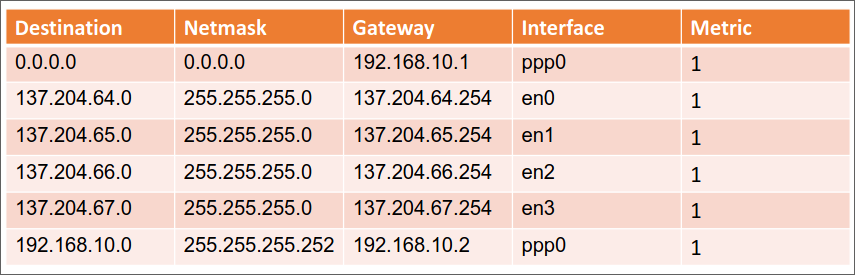
\includegraphics[width=0.9\textwidth]{1/tabR.png}
                \end{figure}
                \subsection{Uso della tabella di routing}
                    Il singolo nodo riceve un datagramma:
                    \begin{itemize}
                        \item Estrae dall'intestazione IP\_D=indirizzo IP di destinazione
                        \item Seleziona il route per tale IP\_D, confrontandolo con i campi D presenti nella tabella, processo di \textbf{table lookup}
                        \item Se il route esiste, esegue l'azione di instradamento suggerita dai campi G e IF, altrimenti genera un messaggio di errore(Tipicamente notificato all'indirizzo sorgente (ICMP-\textbf{Destination Unreachable}
                    \end{itemize}
                \subsection{Table lookup}
                    La ricerca nella tabella avviene confrotando: 
                    \begin{itemize}
                        \item indirizzo di destinazione IP\_D del datagramma
                        \item  destinazione D di ciascun route
                        \item Utilizzando la netmask (N) del route
                    \end{itemize}
                    La procedura viene detta di "longest prefix match":
                    \begin{itemize}
                        \item IP\_D AND N = R : l'indirizzo del datagramma e netmask di ciascuna riga
                        \item R=D : se è uguale la route viene selezionata e il processo termina altrimenti si passa al route successivo
                    \end{itemize}
                    L'ordine di lettura, inizia dalla riga che presenta una netmask con un numero maggiore di bit a 1
                    \begin{figure}[H]
                        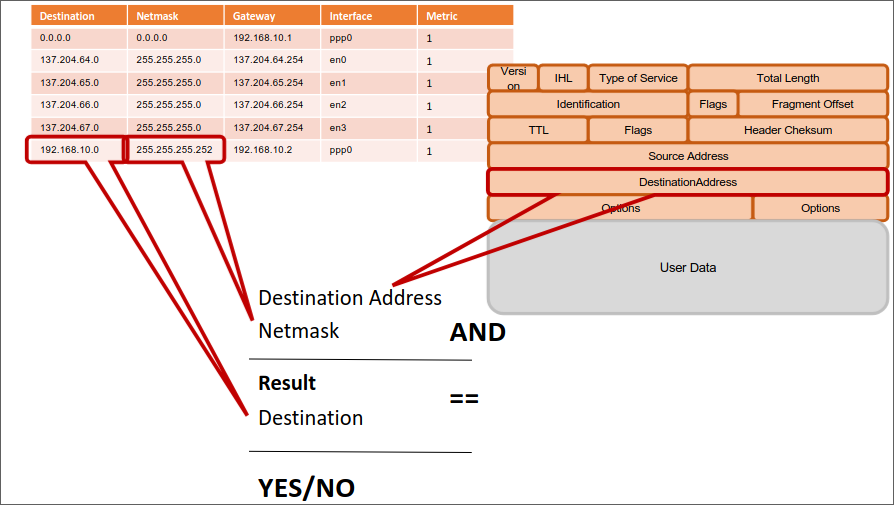
\includegraphics[width=0.9\textwidth]{1/tl.png}
                    \end{figure}
                \subsection{Esempio loock up}
                     \begin{figure}[H]
                        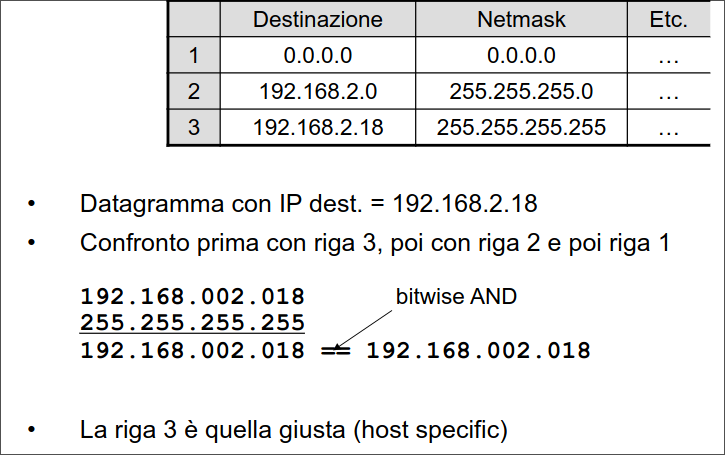
\includegraphics[width=0.9\textwidth]{1/es1.png}
                    \end{figure}
                    \begin{figure}[H]
                        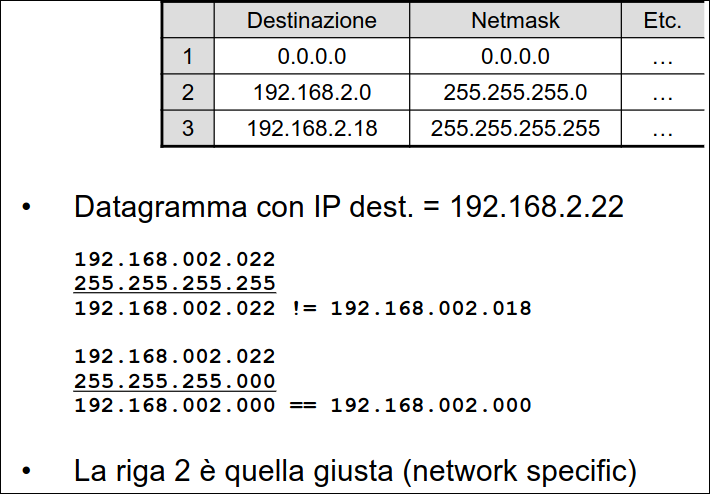
\includegraphics[width=0.9\textwidth]{1/es2.png}
                    \end{figure}
            \subsection{Semplificazione delle tablelle}
                \begin{figure}[H]
                    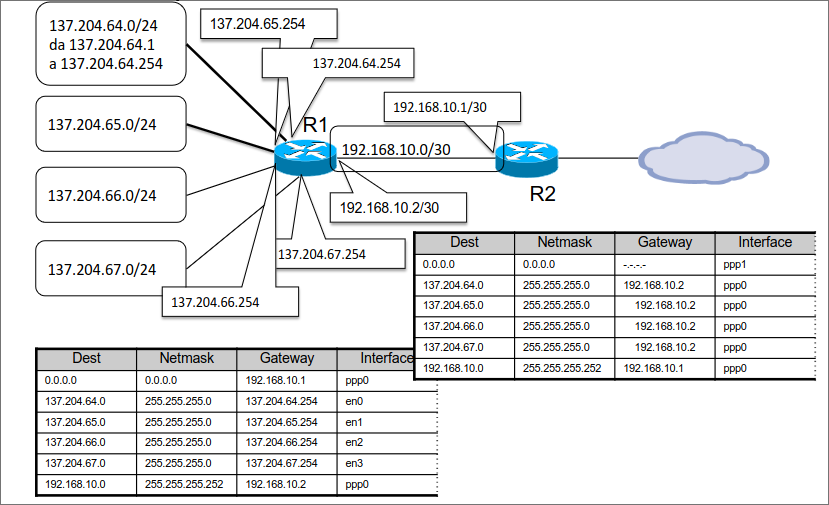
\includegraphics[width=0.9\textwidth]{1/sempTab1.png}
                \end{figure}
                I route verso le 4 network possono essere aggregate in una sola, R2 vede le 4 reti come 1 sola (il gateway verso quelle destinazioni è R1
                 \begin{figure}[H]
                    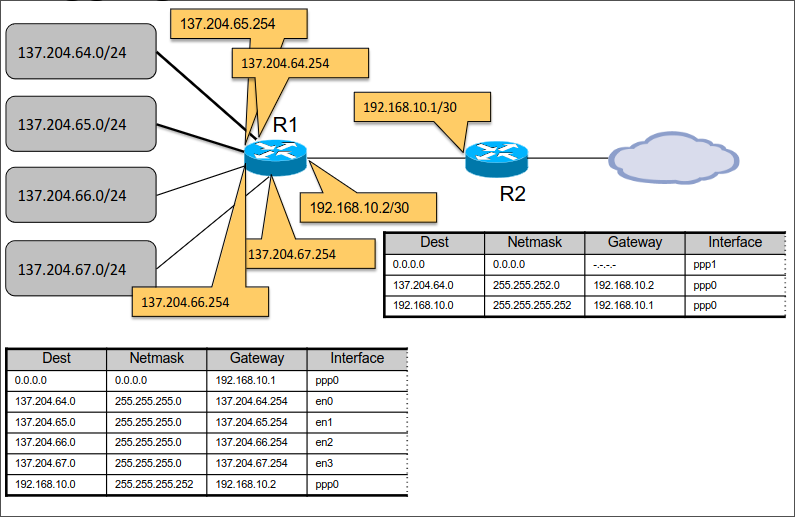
\includegraphics[width=0.9\textwidth]{1/sempTab.png}
                \end{figure}
            \subsection{Perchè ordinare i route}
                Dare priorità alle route più specifiche.
                \\
                L'ordinamento in fnzione della Netmask decrescente garantisce di considerare: singli host, reti piccole, reti grandi.
                \\
                È possibile implementare eccezioni a regole generali che possono convivere nella medesima tablella
                \begin{figure}[H]
                    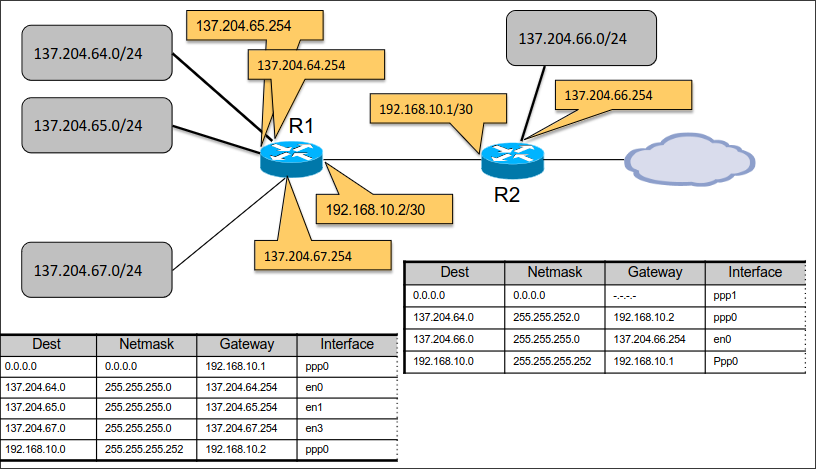
\includegraphics[width=0.9\textwidth]{1/pr.png}
                \end{figure}
                 \begin{figure}[H]
                    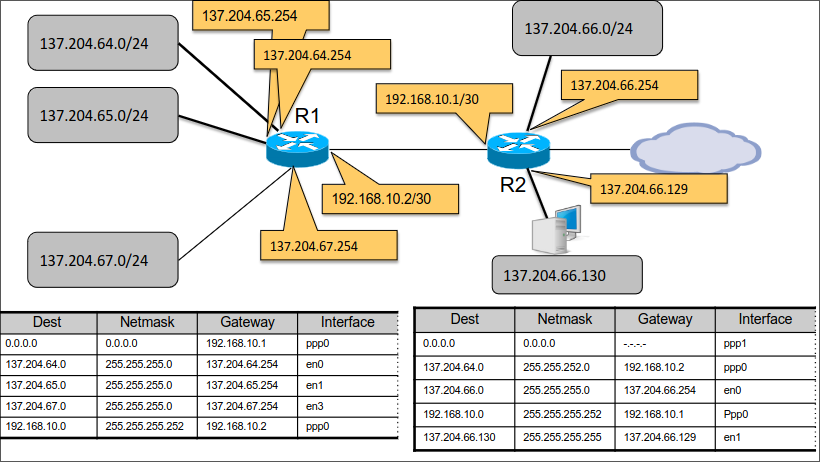
\includegraphics[width=0.9\textwidth]{1/pr2.png}
                \end{figure}
        \section{Gateway}
            Il Gateway è il responsabile della consegna del datagramma.
            \subsection{Il ruolo del gateway}
                Il table look-up sceglie la D i-esima = $D_i$
                \\
                La funzione di instradamento invia il datagramma a $IF_i$, con l'obiettivo di consegnarlo al gateway $G_i$
                \subsubsection{Perchè non è sufficiente $IF_i$?}
                    Perchè l'instradamento IP è basato sull'appartenenza alla network, Host della stessa network possono comunicare direttamente, Host di network diverse comunicano attraverso gateway
            \subsection{Uso del Gateway}
                Il campo gateway della tabella di routing serve per specificare il tipo di instradamento.
                \begin{itemize}
                    \item \textbf{Instradamento diretto} : la sintassi dipende dall'implementazione (In win l'instradamento è locale se gateway=IP locale, in UNIX se = 0.0.0.0
                    \item \textbf{Instradamento indiretto} : Gateway = numero IP del router da contattare 
                \end{itemize}
               \begin{figure}[H]
                    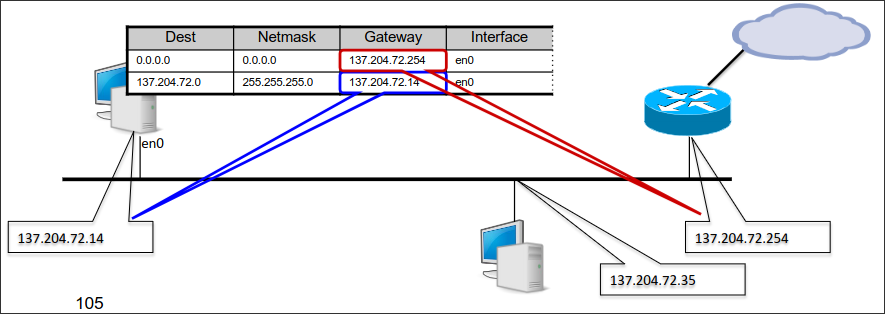
\includegraphics[width=0.9\textwidth]{1/uG.png}
                \end{figure}
    \chapter{La logica degli indirizzi IP}
        \section{IP e Netmask}
            Il numero IP ha valore assoluto in rete, un IP pubblico deve essere unico su Internet, i numeri IP sorgente e destinazione caratterizzano il dtagramma in quanto parte della sua intestazione
            \\
            La netmask:
            \begin{itemize}
                \item relativa al singolo nodo
                \item  non viene trasportata nell'intestazione del dtagramma
                \item è parte della tabella di routing dei singoli nodi
                \item Ai medesimi indirizzi possono corrispondere netmask diverse in nodi diversi (route aggregation)
            \end{itemize}
            Non è sempre stato cosi, inizialmente la suddivisione tra net-ID e host-ID era assoluta
        \section{Classi delle reti}
            Durante a fase iniziale di Internet furono definite diverse "classi" di network differenziate per dimensione
            \\
            La parte iniziale del Net-ID differenzia le classi:
            \begin{itemize}
                \item 0 classe A
                \item 10 classe B
                \item 110 classe C
            \end{itemize}
            La definizione delle classi è stadard e quindi nota a tutti, i router riconoscono la classe di una rete dai primi bit dell'inizio (ricavando di conseguenza il Net-ID)
            \subsection{Classi di Indirizzi}
                \begin{figure}[H]
                    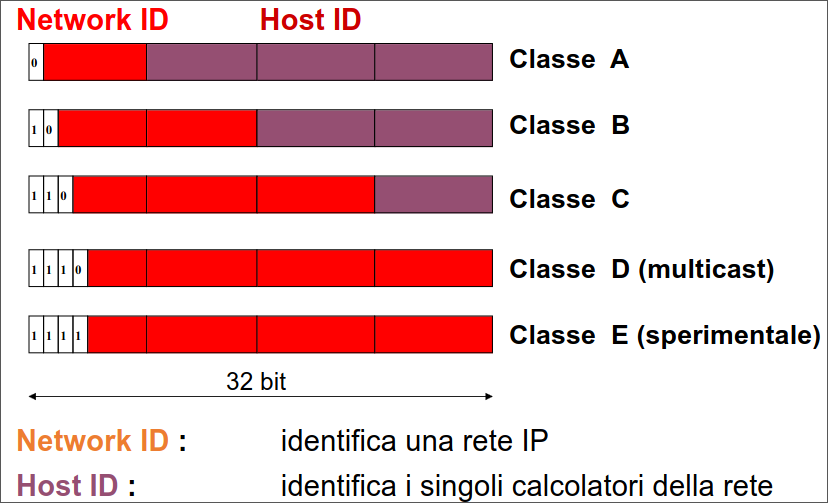
\includegraphics[width=0.9\textwidth]{1/cI.png}
                \end{figure}
            \subsection{Intervalli di Indirizzi}
                \begin{itemize}
                    \item Classe A: da \textbf{0.0.0.0} a \textbf{127.255.255.2255}
                    \item Classe B: da \textbf{191.0.0.0} a \textbf{191.255.255.2255}
                    \item Classe C: da \textbf{192.0.0.0} a \textbf{223.255.255.2255}
                    \item Classe D: da \textbf{224.0.0.0} a \textbf{239.255.255.2255}
                    \item Classe E: da \textbf{240.0.0.0} a \textbf{255.255.255.2255}
                \end{itemize}
            Indirizzi riservati: 
            \begin{itemize}
                \item \textbf{0.0.0.0} : indica l'ost corrente senza specificarne l'indirizzo
                \item HOST-ID tutto a zero : viene usato per indicare la rete
                \item \textbf{0.x.y.z} : indica un certo Host-ID sulla rete corrente senza specificare il Net-ID
                \item \textbf{255.255.255.255} : è l'indirizzo di broadcast su Internet
                \item \textbf{127.x.y.z} : è il loopback, che redirige i datatgrammi agli strati superiori dell'host corrente 
            \end{itemize}
        \section{Le sottoreti}
            A un'amministrazione è assegnata una network, la quale può essere suddivisa in sotto-amministrazioni logicamente separate.
            \\
            Converrebbe quindi "frammentare" la network in "\textbf{sub-network}" da assegnare alle sotto-amministrazioni
            \\
            Si decide localmente una sotto-rpartizione Net/Hpst ID indipendentemente dalle classi. Si frammeta l'Host-ID in due parti:
            \begin{itemize}
                \item la prima identifica la sottorete (subnet-ID)
                \item la seconda iidentifica i singoli host della sottorete
            \end{itemize}
            La ripartizione deve essere locale e reversibile, tutta Internet vede comunque una certa network come entità unitaria
            \subsection{Subnetting}
                La suddivisione è locale alla singola intervaccia (deve essere configurabile localmente)
                \\
                Si personalizza la netmask.
                 \begin{figure}[H]
                    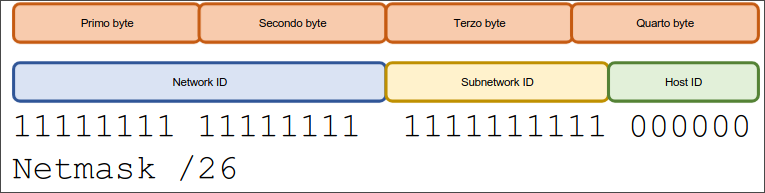
\includegraphics[width=0.9\textwidth]{1/sub1.png}
                \end{figure}
                Subnet diverse essendo Network diverse, hanno bisogno di un gateway per comunicare.
                \begin{figure}[H]
                    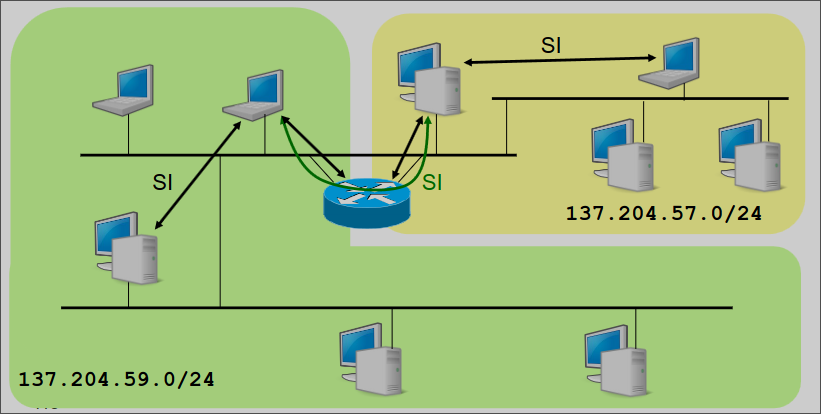
\includegraphics[width=0.9\textwidth]{1/sub2.png}
                \end{figure}
                \subsubsection{Esempio: Università di Bologna}
                    Una network di classe B (137.204.0.0) ha numerose entità distinte nella stessa amministrazione (Facoltà, Dipartimenti ecc..). 
                    \\
                    Si suddivide la network in sottoreti .
                    \\
                    Il primo byte del HOst-ID viene utilizzato come indirizzo di sottorete, dalla network di classe B si ricavano 254 network della dimensione di una classe C,\textbf{ Netmask = 255.255.255.0}
            \subsection{CIDR: Classeless InterDomain Routing}
                Il CIDR rompe la logica delle classi nei router:
                \begin{itemize}
                    \item la dimensione del Net-ID può essere qualunque
                    \item Le tabelle di routing devono comprendere anche la netmask
                    \item Generalizzazione delle subnetting/supernetting (reti IP definite da Net-ID/Netmask)
                \end{itemize} 
                \subsubsection{Obiettivi del CIDR}
                    I suoi obiettivi sono:
                    \begin{itemize}
                        \item Allocazione di reti IP di dimensioni variabili (utilizzo più efficiente degli indirizzi)
                        \item Accorpamento delle informazioni di routing (oiù reti contigue rappresentate da un'unica riga nelle tabelle di routing)
                        \item Miglioramento di due situazioni critiche
                            \begin{itemize}
                                \item Limitatezza di reti di classe A e B
                                \item Crescita esplosiva delle dimensioni delle tabelle di routing
                            \end{itemize}
                    \end{itemize}
            \subsection{Supernetting}
                    Consiste nel raggruppare più reti con indirizzi consecutivi, e indicarle nelle tabelle di routing con una sola entry accompagnata dalla opportuna Netmask.
                    \subsection{Esempio}
                        Un ente ha bisogno di circa 2000 indirizzi IP, una rete di classe B è troppo grande (64k indirizzi, meglio 8 reti di classe C (8 * 256 = 2048 indirizzi) dala 194.24.0.0 alla 194.24.7.0.
                        \\
                        \textbf{Supernetting}: si accorpano le 8 ret contigue in un'unica super-rete: 
                        \begin{itemize}
                            \item Identificativo: 194.24.0.1-194.24.7.254
                            \item Supernet mask: 255.255.248.0
                            \item Indirizzi: 194.24.0.1-194.24.7.254
                            \item Broadcast 194.24.7.255
                        \end{itemize}
                        \subsubsection{Accorpamento}
                            Accorpamento di N reti IP $(N=2^{32})$:
                            \begin{itemize}
                                \item contigue: 
                                \begin{itemize}
                                    \item 194.24.0.0/24+194.24.1.0/24=194.0.0/23
                                    \item 194.24.0.0/24+194.2.0/24=non contigue
                                \end{itemize}
                                \item allineate secondo i multibli di $2^n$: 
                                    \begin{itemize}
                                    \item 194.24.0.0/24+.1.0/24+.2.0/24+.3.0/24=194.24.0.0/22
                                    \item 194.24.0.0/24+.3.0/24+.4.0/24+.5.0/24=non allineate
                                \end{itemize}
                            \end{itemize}
            \subsection{Supernetting e Subnetting}
                subnetting e Supernetting sono operazioni duali:
                \begin{itemize}
                    \item Subnetting: n bit del Host-ID diventano parte del Net-ID
                    \item Supernetting: n bit del Net-ID diventano parte del Host-ID
                \end{itemize}
            \subsection{Oggi}
                La distinzione fra Net-ID e Host-ID è locale funzione della Netmask
                \\
                Lo stesso indirizzo può essere intrpretato in modo diverso in punti diversi della rete
                \\
                Tutte le tabelle di instradamento devono contenere la colonna Netmask
                 \begin{figure}[H]
                    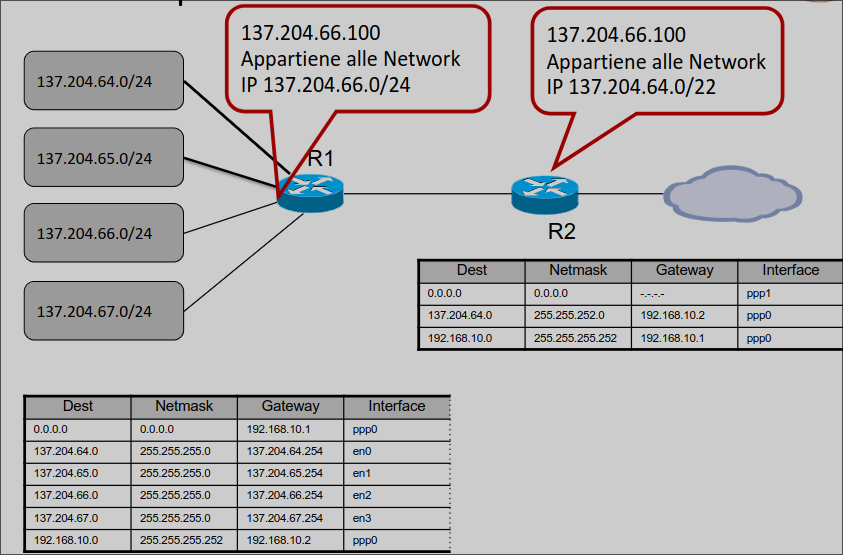
\includegraphics[width=0.9\textwidth]{1/Oggi.png}
                \end{figure}
    \chapter{Protocollo ICMP}
        Il protocollo IP offre un servizio di tipo best effort, quindi non garantisce la corretta consegna dei datagrammi, se necessario si affida a protocolli affidabili di livello superiore.
        \\
        È comunque necessario un protocollo di controllo per :
        \begin{itemize}
            \item gestione di situazioni anomale
            \item notifica di errori o di irraggiungibilità della destinazione 
            \item scabiodi informazioni sulla rete
        \end{itemize}
        \textbf{ICMP}: Internet Control Message Protocol, segnala solamente errori e malfunzionamenti, ma non esegue alcuna correzione, e non rende affidabile l' IP
        \section{Qando viene usato}
            L'IP usa ICMP per la gestione di situazioni anomale, per cui ICMP offre un servizio ad IP.
            \\
            I pacchetti ICMP sono incapsulati in datagrammi IP, per cui ICMP è anche utente IP
            \\
            \begin{figure}[H]
                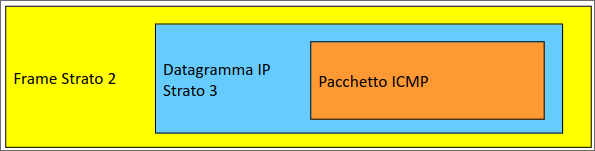
\includegraphics[width=0.9\textwidth]{1/ICMP.png}
            \end{figure}
        \section{Pacchetto ICMP}
            \begin{figure}[H]
                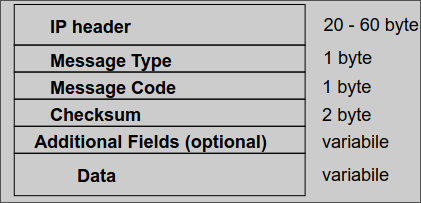
\includegraphics[width=0.9\textwidth]{1/pacICMP.png}
            \end{figure}
            \begin{itemize}
                \item Type : definisce il tipo di messaggio ICMP
                \item Code : descrive il tipo di errore nel messaggio ICMP
                \item Checksum : controlla i bit errati nel messaggio ICMP
                \item Add. Fields : dipendono dal tipo di messaggio ICMP
                \item Data : intestazione a arte dei dati del datagrama che ha generato l'errore
            \end{itemize}
        \section{Tipi di errori}
            \subsection{Destination Unreachable (Type 3)}
                Grenerato da un Gateway quando la sottorete o l'host non sono raggiungibili.
                \\
                Oppure è generato da un host quando si presenta un errore sull'idirizzo dell'entità di livello superiore a cui trasferire il datagramma.
                \subsubsection{Codici di errore}
                    I codici di errore di Destination Unreachable possono essere:
                    \begin{itemize}
                        \item 0 = sorgente non raggiungibile
                        \item 1 = host non raggiungibile
                        \item 2 = protocollo non disponibile 
                        \item 3 = porta non raggiungibile 
                        \item 4 frammentazione necessaria ma bit don't fragment settato
                    \end{itemize}
            \subsection{Time Exceeded (Type = 11)}
                È generato da un router quando il Time-to-Live di un datagramma si azzera ed il datagramma viene distrutto (Code = 0).
                \\
                Oppure viene generato da un HOst quando un timer si azzera in attesa dei frammenti per riassemblare un datagramma ricevuto in parte (Coe = 1)
            \subsection{Surce Quench (Type = 4)}
                I datagrammi arrivano troppo velocemente rispetto alla capacità di essere processati: l'host sorgente deve ridurre la velocità di trasmissione (obsoleto)
            \subsection{Redirect (Type = 5)}
                Generato da un router per indicare all'host sorgente un'altra strada più conveniente per raggiungere l'host destinazione
                
        \section{Informazioni}
            \subsection{Echo (Type=8) / Echo Reply (Type = 0)}
                L'host sorgente invia la richiesta ad un altro host o ad un gateway., la destinazione deve risondere.
                \\
                Questo metodo è usato per determinare lo stato di una rete e dei suoi host, la loro raggiungibilità e il tempo di transitonella rete
            \subsection{Additional Fields}
                Identifier : identifica l'insieme degli echo appartenenti allo stesso test.
                \\
                Sequence Number : identifica ciascun echo nell'insieme 
                \\
                Optional Data : usato per inserire eventuali dati di verifica
            \subsection{Timestamp Request (Type = 13) / Reply(Type = 14)}
                L'host sorgente invia all'host destinazione un Originale Timestamp che indica l'istante in cui la richiesa è partita
                \\
                L'host destinazione risponde inviando un:
                \begin{itemize}
                    \item Recive Timestamp che indica l'istante che indica in cui la richiesta è stata ricevuta
                    \item Transmit Timestamp che indica l'istante in cui la risposta è stata inviata
                \end{itemize}
                Serve per valutare il tempo di transito nella rete, al netto del tempo di processamento =$T_{Transmit}-T_{Receive}$
            \subsection{Address Mask Request (Type = 17) / Reply (Type = 18)}
                Inviato dall'host sorgente all'indirizzo di broadcast (255.255.255.255)
                per ottenere la subnet mask da usare dopo aver ottenuto il proprio indirizzo IP tramite RARP o BOOTP
            \subsection{Router Solicitation (Type = 10)} 
            \subsection{Router Advertisement (Type = 9)}
                Utilizzato per localizzare i router connessi alla rete
    \chapter{Applicazioni di ICMIP}
        \section{PING}
            Il comando ping DEST permette di controllare se l'host DEST è raggiungibile o meno dalla sorgente (SORG
            \begin{figure}[H]
                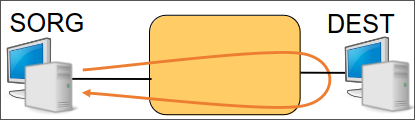
\includegraphics[width=0.9\textwidth]{2/ping.png}
            \end{figure}
            %TODO comando pic es
            \subsection{funzionamento}
                SORG invia a DEST un pacchetto ICMP di tipo "echo", se l'host DEST è raggungibile da SORG, dest risponde inviando indietro un pacchetto ICMP di tipo "echo reply"
            \subsection{Opzioni}
                \begin{itemize}
                    \item \textbf{-n N} : permette di specificare quanti pacchetti inviare (un pacchetto al secondo)
                    \item \textbf{-l M} specifica la dimensione in byte di ciascun pacchetto
                    \item \textbf{-t} : esegue il ping finchè interrotto con Ctrl-C
                    \item \textbf{-a} : traduce l'indirizzo IP in nome DNS
                    \item \textbf{-f} : setta il bit dont'fragment a 1
                    \item \textbf{-i T} : setta time-to-live = T
                    \item \textbf{w $T_{out}$} : specifica un timeout in millisecondi
                \end{itemize}
            \subsection{Output}
                L'output mostra: 
                \begin{itemize}
                    \item la dimensione del pacchetto "echo reply"
                    \item l'indirizzo IP di DEST
                    \item il numero di sequenza della risposta
                    \item il "time-to-live" TTL
                    \item il "rount-trip time" (RTT)
                    \item alcuni risultati statistici: N° pacchetti persi, MIN, MAX e media del RTT
                \end{itemize}
            \subsection{Traceroute}
                Il comando \textbf{tracert DEST} permette di conoscere il percorso seguito dai pacchetti inviati da SORG e diretti verso DEST
                \begin{figure}[H]
                    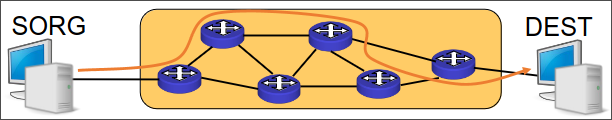
\includegraphics[width=0.9\textwidth]{2/trace.png}
                \end{figure}                
            \subsection{Funzionamento}
                    \begin{enumerate}
                        \item SORG invia a DEST una serie di pacchetti ICMP di tipo ECO con un TIME-TO-LIVE progressivo da 1 a 30 (per default
                        \item Ciscun nodo intermedio decrementa TTL
                        \item Il nodo che rileva TTL=0 invia a SORG un pacchetto ICMP di tipo TIME EXCEEDED
                        \item SORG costruisce una lista dei nodi attraversati fino a DEST
                    \end{enumerate}
                \subsection{Output}
                    L'output mostra il TTL, il nome del DNS e l'indirizzo IP dei nodi intermedi ed il ROUND-TRIP-TIME (RTT)
    \chapter{Gestione della enumerazione}   
        \section{Dispositivi di rete}
            \subsection{DHCP}
                Il DHCP permette ad un Host di ottenere una configurazione IP.
                \\
                Consente la configurazione automatica e dinamica di:
                \begin{itemize}
                    \item Indirizzo IP
                    \item Netmask
                    \item Host name
                    \item Default gateway
                    \item Server DNS
                \end{itemize}
                Server su porta 67 UDP
                \subsubsection{Funzionamento}
                    Quando l'host attiva l'interfaccia di rete, invia in modalità broadcast un messaggio \textbf{DHCPDISCOVER} in cerca di un server DHCP
                    \begin{figure}[H]
                        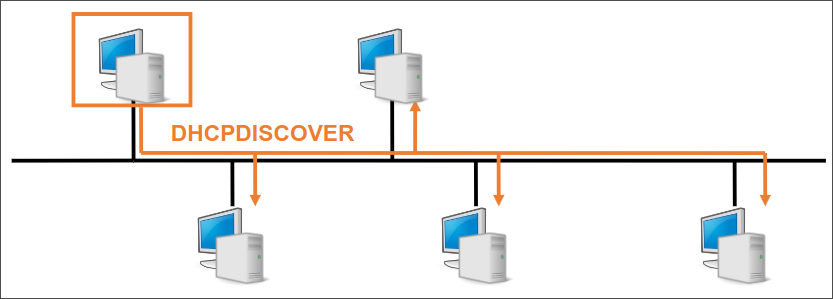
\includegraphics[width=0.9\textwidth]{2/DHCP1.png}
                    \end{figure}
                    Ciscun server DHCP persente risponde all'host con un messaggio \textbf{DHCPOFFER} con cui propone un indirizzo IP
                    \begin{figure}[H]
                        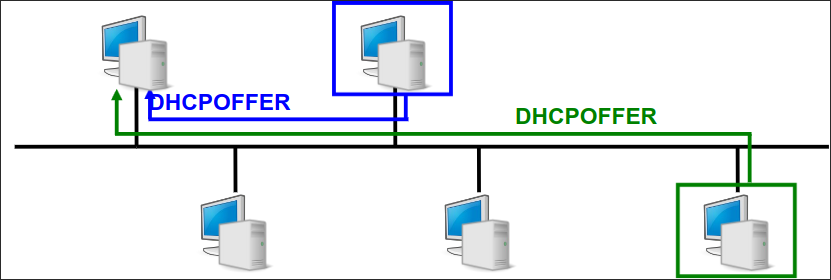
\includegraphics[width=0.9\textwidth]{2/DHCP2.png}
                    \end{figure}
                    L'host accetta una delle offerte proposte dal server e manda un messaggio \textbf{DHCPREQUEST} in cui chiede la configurazione, specificando il server
                    \begin{figure}[H]
                        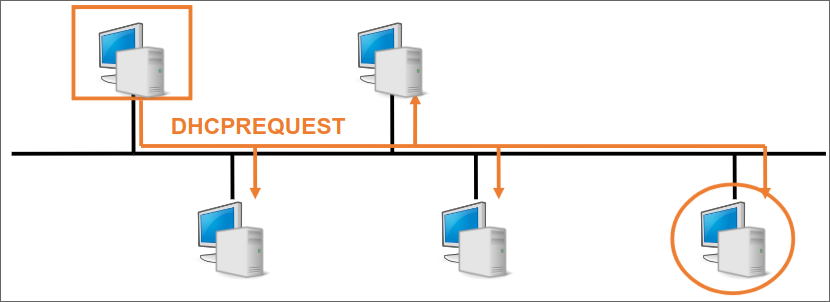
\includegraphics[width=0.9\textwidth]{2/DHCP3.png}
                    \end{figure}
                    Il server DHCP risponde con un messaggio \textbf{DHCPACK} specificando i parametri di configurazione
                    \begin{figure}[H]
                        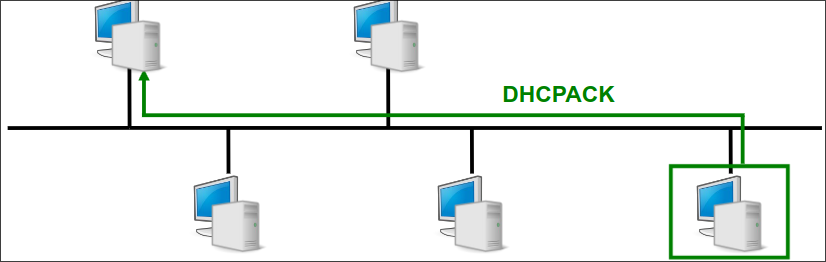
\includegraphics[width=0.9\textwidth]{2/DHCP4.png}
                    \end{figure}
            \subsection{Packet Filter}
                Il Packet Filter permette o blocca l'invio di pacchetti da e veroso determinati indirizzi, e protegge la rete dal traffico "vagante"
            \subsection{Application Layer Gateway (ALG) / Proxi}
                Il Proxi controlla la comunicazione a livello applicativo
            \subsection{Firewall}
                Il Firewall, è la combinazione dei precedenti dispositivi, e serve per proteggere le risorse interne da accessi esterni
            \subsection{Network Address Translator (NAT)}
                Il NAT riduce la richiesta dello spazio di indirizzamento Interne, nasconte gli indirizzi IP interni e esegue un packet filtering per il traffico sconosciuto
    \chapter{Packet Filter e Firewall}
        \begin{figure}[H]
            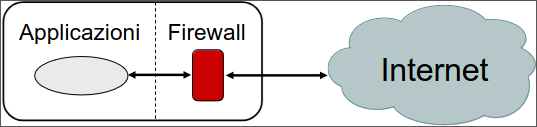
\includegraphics[width=0.9\textwidth]{2/fir.png}
        \end{figure}
        \section{Firewall}
            \subsection{Packet filter} 
                IL packet filter filtra i pacchetti seguendo le politiche stabilite :
                \begin{itemize}
                    \item Filtri: generalmente configurati staticamente
                    \item La maggioranza delle configurazioni non permettono pacchetti per porte "non-standar" (Internet Assigned Numbers Autority - IANA)
                \end{itemize}
            \begin{figure}[H]
                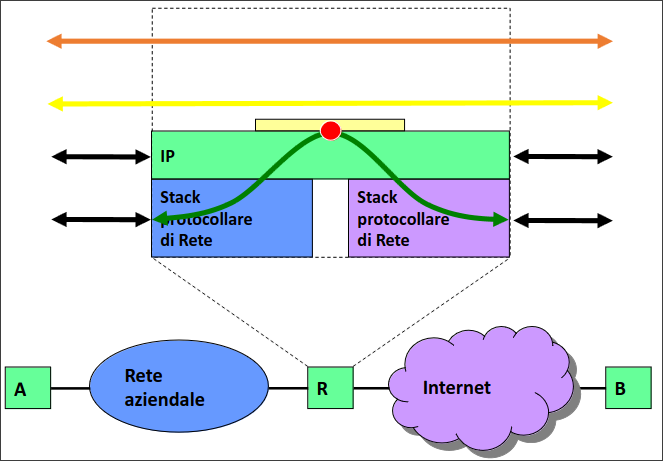
\includegraphics[width=0.9\textwidth]{2/pac.png}
            \end{figure}
            \subsection{Stateful Packet Inspection}
                Mantiene l contesto dei pacchetti sia nel trasporto che nello strato applicativo, e adatta dinamicamente le specifiche dei filtri.
                \begin{figure}[H]
                    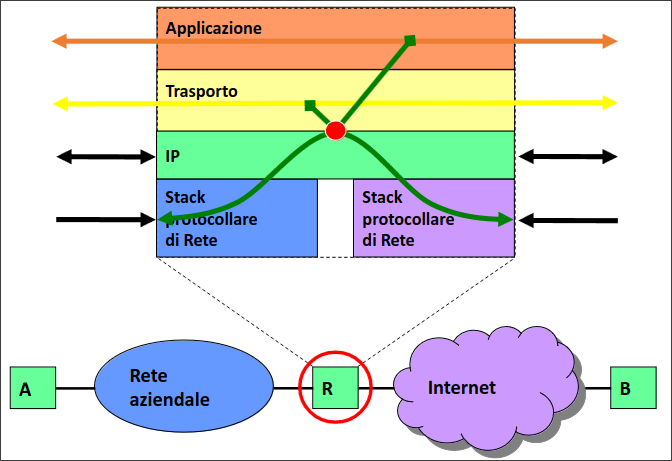
\includegraphics[width=0.9\textwidth]{2/stateFull.png}
                \end{figure}
            \subsection{Application Layer Gateway (trasparente o proxy esplicito)}
                Monitora le conessioni: analizza il contenuto dei protocolli applicativi, a scapito della sicurezza di comunicazione end-to-end.
                \\
                Adatta dinamicamente le specifiche dei filtri.
                \begin{figure}[H]
                    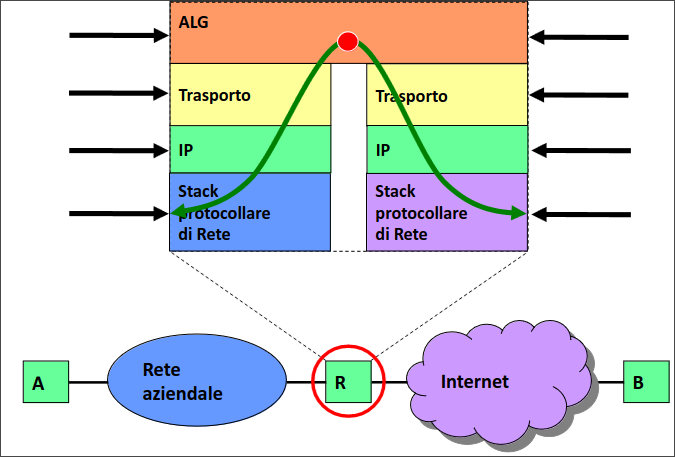
\includegraphics[width=0.9\textwidth]{2/apL.png}
                \end{figure}
                \begin{figure}[H]
                    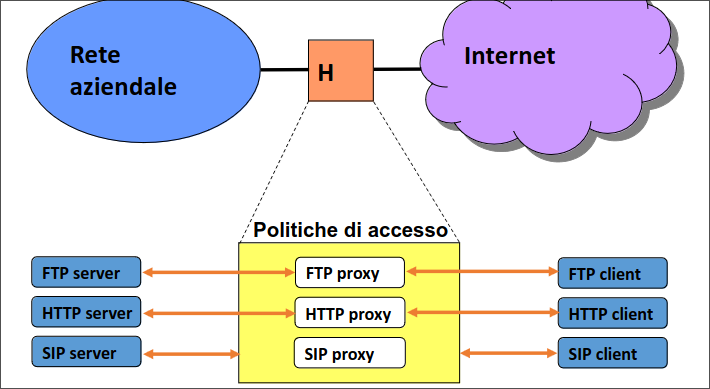
\includegraphics[width=0.9\textwidth]{2/apL2.png}
                \end{figure}
        \section{Protezione Host: firewall}
            Un firewall è un filtro software/hardware che serve a proteggersi da accessi indesiderati provenienti dall'esterno della rete.
           \\
            Può essere semplicemente un programma installato sul proprio PC che protegge quest'ultimo da attacchi esterni. Tipicamente è usato in accessi domestici a larga banda (ADSL, FTTH).
            \\
            Oppure può essere una macchina dedicata che filtra tutto il traffico da e per una rete locae
            \begin{figure}[H]
                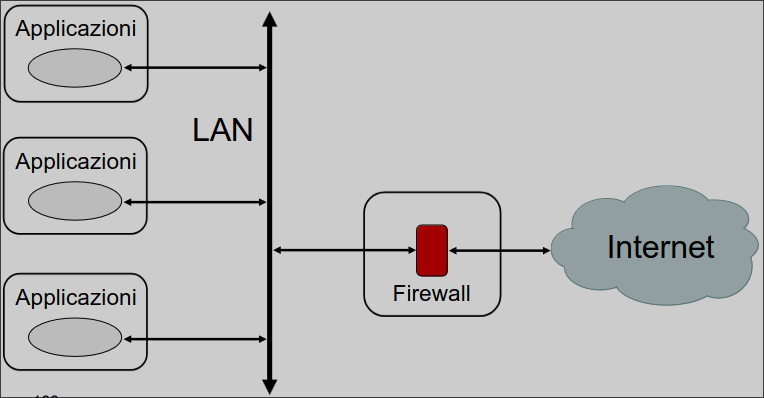
\includegraphics[width=0.9\textwidth]{2/fir2.png
                }
            \end{figure}
            Tutto il traffico fra la rete locale ed Internet deve essere filtrato dal firewall, e solo il traffico autorizzato deve attraversare il firewall.
            \\
            Ma si devecomunque permettere che i servizi di rete ritenuti necessari siano mantenuti.
            \\
            Il firewall deve essere per quanto possibile immune da problemi di sicureza sull'host
            \\
            In fase di configurazione di un firewall, per prima cosa si deve decidere la politica di default per i servizi di rete:
            \begin{itemize}
                \item \textbf{default deny} : tutti servizi non esplicitamente permessi sono negati
                \item \textbf{default permit} : tutti i servizi non esplicitamente negati sono permessi
            \end{itemize}
        \section{Livelli di implementazione}
            Un firewall può essere implementato come: 
            \begin{itemize}
                \item packet filter 
                \item proxi server
                \begin{itemize}
                    \item application gateway
                    \item circuit-level gateway
                \end{itemize}
            \end{itemize}
            \subsection{Packet Filter}
                Si interpone un router fra la rete locale e internet, sul router si configura un filtro sui datagrammi IP da trasferire attraverso le varie interfaccie, il fltro scarta i datagrammi sulla base di :
                \begin{itemize}
                    \item indirizzo IP sorgente e destinazione
                    \item tipo di servizio a cui il datagramma è destinato (perta TCP/UDP)
                    \item interfaccia di provenienza o destinazione
                \end{itemize}
            \subsection{Proxy server0}
                Nella rete protetta l'accesso ad internet è consentito solo ad alcuni host.
                \\
                Si interpone un server apposito detto proxy server per realizzare la comunicazione per tutti gli host
                \\
                Il proxy server evita un flusso diretto di datagrammi fra Internet e le macchine della rete locale.
                \\
                \subsubsection{Application level}
                    Viene impiegato un proxy server dedicato per ogni servizio che si vuole garantire
                \subsubsection{Circuit level gateway}
                    È un proxy server generico in grado d inoltrare le richieste relative a molti servizi
        \section{Configurazione di packet filter e proxy}
            \begin{figure}[H]
                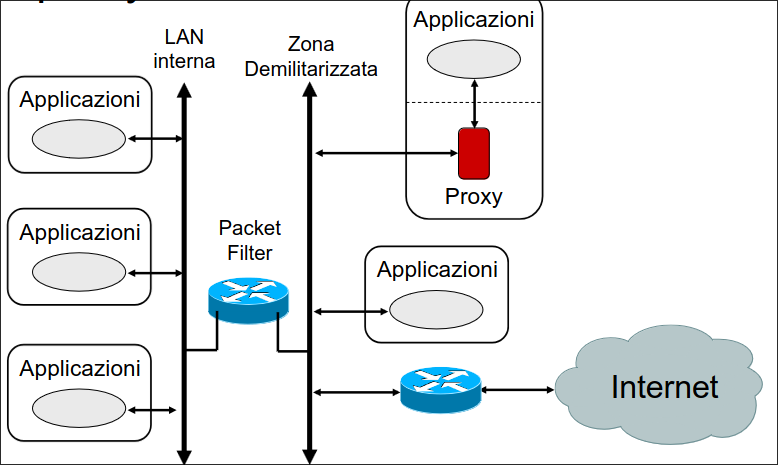
\includegraphics[width=0.9\textwidth]{2/confPac.png}
            \end{figure}
    \chapter{Network Address Translation}
        Tecnica per il filtraggio di pacchetti IP con sostituzione degli indirizzi (mascheramento).
        \\
        Permette a IP private l'accesso a reti IP pubbiche tramite un appoito gateway, è utile per ripiarmiare indirizzi IP pubblici e il riutilizzo di indirzzi IP privati 
        \begin{figure}[H]
            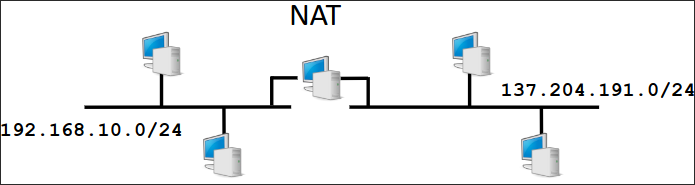
\includegraphics[width=0.9\textwidth]{2/NAT.png}
        \end{figure}
        \section{Motivazioni}
            \begin{itemize}
                \item Efficiente uso dello pazio degli indirizzi
                \item Condividere uno o pochi indirizzi
                \item Uso di indirizzi privati nella LAN locale (10.x.x.x., 192.168.x.x, ..)
                \item  Rende gli host interni non accessibili dall'esterno
                \item Include un packet filter, stateful packet inspection configurati dinamicamente
            \end{itemize}
        \section{Network (+Port) Address Translator (NAT)}
            \begin{figure}[H]
                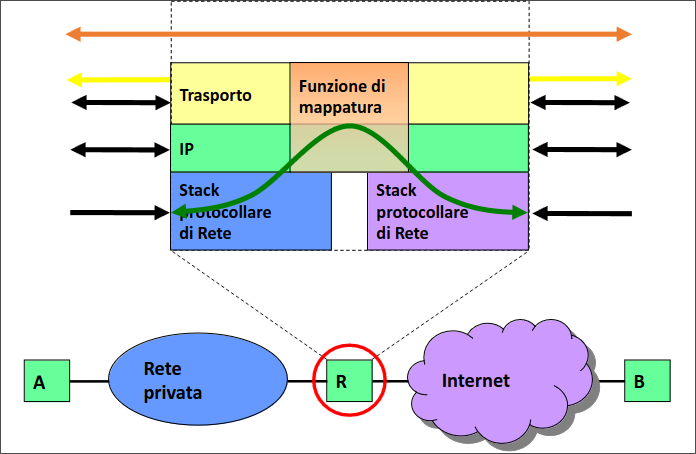
\includegraphics[width=0.9\textwidth]{2/NAT2.png}
            \end{figure}
        \section{Basic Nat}
            \subsection{Conversione di Indirizzo}
                Il NAT può fornire una semplice conversione di indirizzo IP (statica o dinamica).
                \\
                Conversioni conteporaneaente limitate dal numero di indirizzi IP pubblici a disposizione del gateway NAT
                \begin{figure}[H]
                    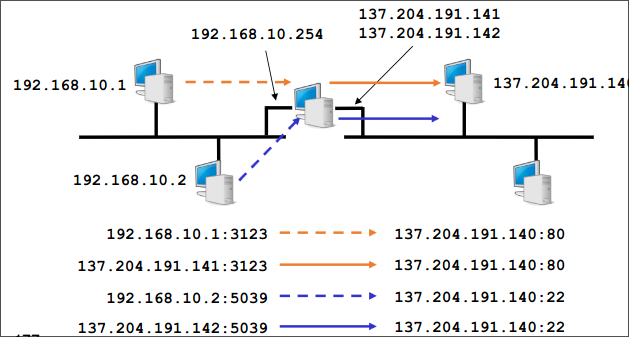
\includegraphics[width=0.9\textwidth]{2/convInd.png}
                \end{figure}
            \subsection{Conversione di indirizzo e porta}
                Il NAT può fornire anche la conversione di indirizzo IP e porte TCP o UDP.
                \\
                Le conversioni contemporanee sono possibili anche con un unico indirizzo IP pubblico del gateway NAT 
                \begin{figure}[H]
                    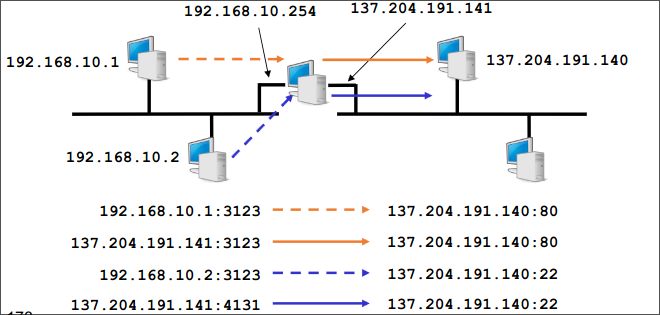
\includegraphics[width=0.9\textwidth]{2/pc.png}
                \end{figure}
            \subsection{Direzione delle connessioni}
                La direzione delle connessioni sono tipicamente da rete privata verso rete pubblica.
                \\
                Il NAT si preoccupa di effetuare la conversione inversa quando arrivano le risposte, e registra le corrispondenze in corso in una tabella.
                \\
                È anche possibile contattare dalla rete ubblica un host sulla rete privata se il tipo di NAT e la relativa configurazione lo permette.
               \begin{figure}[H]
                    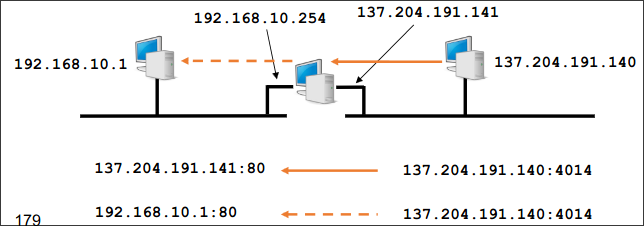
\includegraphics[width=0.9\textwidth]{2/dirc.png}
                \end{figure}
            \subsection{Port forwarding}
                Il NAT permette l'ingresso di pacchetti estinati a porte specifiche effettuando la traduzione opportuna.
                 \begin{figure}[H]
                    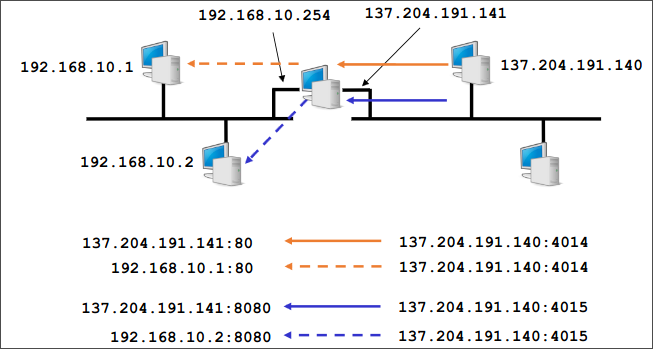
\includegraphics[width=0.9\textwidth]{2/portFor.png}
                \end{figure}
            \subsection{Analisi di connessioni attraverso NAT}
                \begin{figure}[H]
                    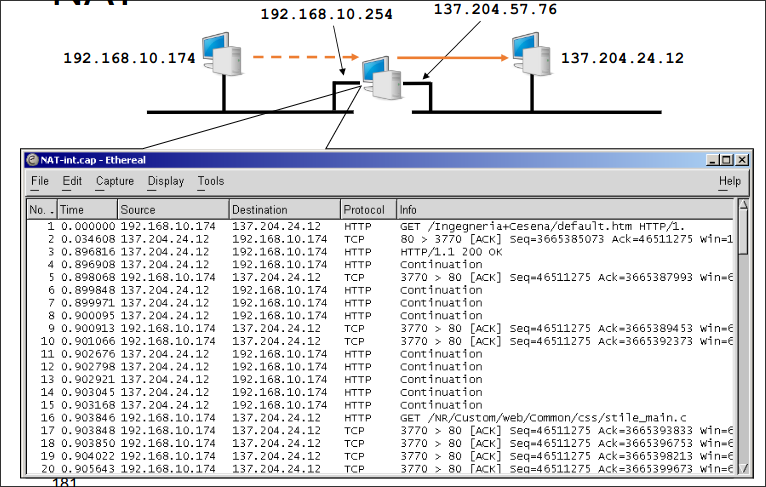
\includegraphics[width=0.9\textwidth]{2/an1.png}
                \end{figure}
                \begin{figure}[H]
                    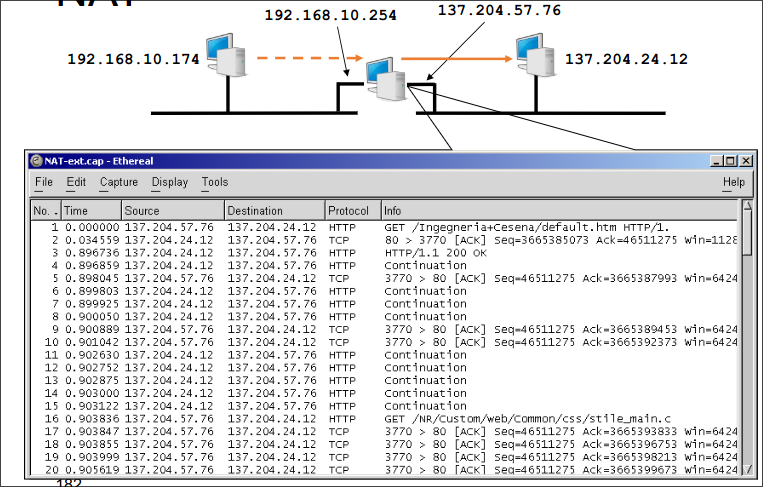
\includegraphics[width=0.9\textwidth]{2/an2.png}
                \end{figure}
        \section{NAT e applicazioni di rete}
            Il NAT è trasparente per l'applicazione, modifica l'intestazione IP e TCP/UDP ma non il payload.
            \\
            Questo potrebbe essere un problema in alcuni casi specifici:
            \subsection{Le applicazioni non sono trasparenti al NAT}
                Contengono indirizzi IP e payload.
                \\
                FTP utilizza due connessioni parallele:
                \begin{itemize}
                    \item connessione per l'intestazione con il server tramite linea di comando 
                    \item connessione per il trasferimento dei dati da e verso il server
                    \item i parametri della seconda sono specificati dai dati della prima
                \end{itemize}
            \subsection{Il tipo di traffico permesso dipende dal ipo di nat}
                \begin{itemize}
                    \item Full Cone NAT
                    \item (Port) Restricted Cone NAT
                    \item Symmetric NAT
                \end{itemize}
    \chapter{IPv6}
        \section{Problematiche dell'indirizzamento IP}
            \begin{itemize}
                \item Mobilità :
                    \begin{itemize}
                        \item Indirizzi riferiti alla rete di appartenenza
                        \item Se un host viene spostato in un'altra rete, il suo indirizzo IP deve cambiare (configurazione automatica con DHCP, mobile IP)
                    \end{itemize}
                \item Sicureza :
                    \begin{itemize}
                        \item Scarsa protezione del datagramma IP (intestazione in chiaro), IPsec applicabile anche a IPv4
                    \end{itemize}
                \item Dimensioni della rete prefissate :
                    \begin{itemize}
                        \item subnetting e CIDR
                    \end{itemize}
                \item Data l'enorme diffusione di Interne, il numero di indirizzi possibili è troppo basso (Reti IP private NAT)
            \end{itemize}
        \section{Soluzione: IPPv6}
            Dati i problemi dell'IPv4 si è lavorato su una nuova versione con i seguent obiettivi: 
            \begin{itemize}
                \item Supportare molti miliardi di host
                \item Semplificare il routing
                \item Offrire meccanismi di sicurezza
                \item Offrire qualità di servizio (multimedialità)
                \item Gestire bene ulticast e breadcast
                \item Consentire la mobilità
                \item Fare tutto questo consentendo future evoluzioni e garantendo compatibilità con il passato
            \end{itemize}
    \chapter{Instradamento nelle reti a pacchetto e in Internet}
        \section{Funzioni dell' IP}
            \begin{itemize}
                \item Indirizzamento
                \item Frammentazione
                \item Instradamento
                    \begin{itemize}
                        \item Decidere che percorso un datagramma deve seguire per raggiungere la destinazione alla sorgente
                        \item Utilizza le PCI dei datagrammi, in particolare l'indirizzo destinazione
                        \item Determina il comportamento della funzione di commutazione
                    \end{itemize}
            \end{itemize}
            Il problema dell'instradamento è più generale rispetto allo specifico protocollo di livello 3
        \section{Il nodo di commutazione a pacchetto}
            \begin{figure}[H]
                \includegraphics[width=0.9\textwidth]{3/nCp.png}
            \end{figure}
            \subsection{Store-and-Forward}
                Il pacchetto è verificato e memorizzato, si estraggono le informazioni di instradamento dall'intestazione(indirizzo, priorità, casse di servizio).
                \\
                Si confrontano queste informazioni con la tabella di instradamento, identificando una o più uscite su cui inviare il pacchetto.
                \\
                Il pacchetto è inserito nella coda relativa all'uscita prescelta, in attesa della effettiva trasmissione. IL pacchetto viene prima memorizzato interamennte nel nodo e quindi ritrasmesso nella direzione opportuna.
                \\
                In generale dovrebbe esistere una base dati per il confronto che è la tabella di instradamento
        \section{Flooding}
            La soluzione più semplice è il flooding.
            \\
            È molto adatto quando si desidera inviare una certa informazione a tutti i nodi della rete (broadcasting)
            \subsection{Funzionamento}
                Ogni nodo ritrasmette su tutte le porte di uscita ogni pacchetto ricevuto.
                \\
                Prima o poi un pacchetto viene ricevuto da tutti i nodi della rete e quindi anche da quello a cui è effitivamente destinato.
                \\
                Il primo pacchetto che arriva a destinazione ha fatto la strada più breve possibile.
                \\
                L'elaborazione associata è pressochè nulla.
            \subsection{Problema}
                IL problema è la proliferazione di pacchetti, perchè nel singolo nodo ogni pacchetto viene copiato tante volte quante sono le intrfacce, e se è ritrasmesso sull'interfaccia da cui è arrivato il numero di copie cresce esponenzialmente
            \subsection{Soluzione}
                Le soluzioni potrebbero essere:
                \begin{itemize}
                    \item un nodo non può ritrasmettere il pacchetto nella direzione dalla quale è giunto
                    \item ad ogni pacchetto viene associato un identificativo unico (l'indirizzo della sorgente e un numero di sequenza) e ciascun nodo mantiene in memoria una lista con gli identificativi dei pacchetti già trasmessi
                    \begin{itemize}
                        \item Il nodo crea una lista dei pacchetti ricevuti e trasmessi
                        \item  Ogni pacchetto già trasmeso, viene ignorato
                        \item Ogni pacchetto viene ritrasmesso da ogni nodo una sola volta
                    \end{itemize}
                    \item Contatore del tempo di vita (TTL) di un pacchetto per evitare che giri all'infinito
                \end{itemize}
        \section{Deflection routing (hot potato)}
            Nel Deflection routing qando un nodo riceve un pacchetto lo ritrasmette sulla linea d'uscita avente il minor numero di pacchetti in attesa di essere trasmessi
            \subsection{Per quali reti è adatto?}
                È adatto a reti in cui, i nodi di commutazione dispongono di spazio di memorizzazione molte limitato, e se si desidera minimizzare il tempo di permanenza dei pacchetti nei nodi
            \subsection{Propblemi}
                I pacchetti possono essere ricevuti fuori sequenza, e alcuni pacchetti potrebbero percorrere all'infinito un certo ciclo interno alla rete, semplicemente perchè le sue linee sono poco utilizzate
            \subsection{soluzioni}
                Si deve prevedere un meccanismo per limitare il tempo di vita dei pacchetti.
                \\
                Non tiene conto della destinazione finale
        \section{Shortest path routing}
            Si assume che ad ogni collegamento della rete possa essere attribuita una lunghezza.
            \\
            la \textbf{lunghezza} è un numero che serve a caratterizzare il peso di quel collegamento nel determinare la funzione di costo del percorso totale di trasmissione.
            \\
            L'algoritmo cerca la strada di lunghezza minima fra ogni mittente e ogni destinatario.
            \\
            Si applicano algoritmi di calccolo dello shortest path (Bellman Ford e Dijktra).
            \subsection{Iplementazione}
                L'impementazione può essere:
                \begin{itemize}
                    \item Centralizzata: un solo nodo esegue i calcoli per tutti
                    \item Distribuita :
                        \begin{itemize}
                            \item  Ogni nodo esegue i calcoli per se
                            \item Sincrona : tutti i nodi eseguono gli stessi passi dell'algoritmo nello stesso istante
                            \item Asincrona : i nodi eseguono lo stesso passo dell'algoritmo in momenti diversi
                        \end{itemize}
                    \end{itemize}
        \section{Rappresentazione della rete}
            Ad una generica rete di telecomunicazione si può associare un grafo orientato
            \\
            Nel quale, 
            \begin{itemize}
                \item i nodi rappresentano i terminali ed i commutatori
                \item  gli archi rappresentano i collegamenti
                \item L'orientamento degli archi rappresenta la direzione di trasmissione
                \item il peso degli archi rappresenta il costo dei collegamenti, che può essere espresso in termni di:
                \begin{itemize}
                    \item numero di nodi attraversati (ogni arco ha peso unitario)
                    \item distanza geografica
                    \item ritardo introdotto dal collegamentoà
                    \item ritardo introdotto dal collegamento
                    \item inverso della capacitò del collegamento 
                    \item costo di un certo instradamento
                    \item una combinazione dei precedenti
                \end{itemize}
            \end{itemize} 
        \section{Il grafo della rete}
            Una rete è un insieme di nodi di commutazione interconnessi da collegamenti.
            \\
            Per rappresentarla si possono usare i modelli matematematici della teoria dei grafi:
            \begin{itemize}
                \item Sia V un insieme finito di nodi 
                \item Un arco è definito come una coppia di nodi $(i,j), i,j\in V$
                \item Sia E un insieme di archi
                \item Un grafo G è definito come la coppia $V,E)$ e può essere:
                \begin{itemize}
                    \item Orientato se E consiste di coppie unitarie, cioè se $(i,j)\ne (j,i)$
                    \item non-orientato: se E consiste in coppie non ordinate, cioè se  $(i,j)=(j,i)$
                \end{itemize}
                \item  Se $(i,j)\in E$, il nodo $ j$ è vicino del nodo $i$
            \end{itemize}
        \section{Routing shortest path nel mondo IP}
            Quando i nodi di rete vengono accesi conoscono solamente la configurazione delle loro interfacce, statica o dinamica con il DHCP.
            \\
            Con queste informazioni popolano la tabella di instradamento iniziale.
            \\
            Per implementare il routing shortest path verso una qualunque destinazioe devono utilizzare:
            \begin{itemize}
                \item Uno o piùprotocolli di routing per scambiarsi informazioni ed apprendere la tecnologia della rete
                \item Uno o più algoritmi per il calcolo degli SP sulla base delle informazioni
            \end{itemize}
        \section{Rouing distance vector}
            È basato su Bellman-Ford, in versione dinamica e distribuita (proposta da Ford-Fulkerson).
            \\
            È un protocollo semplice che richiede poche risorse.
            \subsection{Cosa implementa}
                Implementa meccanismi di dialogoo per fare si che:
                \begin{itemize}
                    \item gni nodo scopre i suoi vicini e ne calcola la distanza da se stesso
                    \item e che ad ogni passo, ogni nodo invia ai propri vivcini un vettore contenente la stima della sua distanza da tutti gli altri nodi della rete (quelli di cui è a conoscenza)
                \end{itemize}
            \subsection{Problemi}
                Ha una convergenzae una partenza(cold start) lenta, inoltre ha problemi di stabilità, in quanto pùò portare al conteggio infinito
            \subsection{Esempio}
                \begin{figure}[H]
                    \includegraphics[width=0.9\textwidth]{3/esDV.png}
                \end{figure}
            \subsection{}{Cold start e tempo di convergenza}
                Allo start-up le tabelle dei singoli nodi contengono solo l'indicazioni del nodo stesso a distanza 0 (i distance vector scambiati al primo passo contengono solo queste informazioni).
                \\
                Da qui in poi lo scambio dei distance vector permette la creazione di tabelle sempre più complete. L'algoritmo converge al più dopo un numero di passi pari al numero di nodi della rete.
                \\
                Se la rete è molte grande il tempo di convergenza può essere lungo.
                \subsubsection{Cosa succede se lo stato della rete cambia in un tempo inferiore a quello di convergenza dell’algoritmo?}
                    Il risultato diventa imprevedibile e si ritarda la convergenza
            \subsection{Bouncing effect}
                Il link tra due nodi A e B cade,  A e B si accorgono che il collegamento non funziona e immediatamente pongono ad infinito la sua lunghezza.
                \\
                Se altri nodi hanno nel frattempo inviato anche i loro vettori delle distanze, si possono creare delle incongruenze temporane, di durata dipendente dalla complessità della rete, ad esempio A crede di poter raggiungere B tramite un altro nodo C che a sua volta passa attraverso A
                \\
                Queste incongruenze possono dare luogo a cicli, per cui due o più nodi si scambiano datagrammi fino a che non si esaurisce il TTL o finchè non si converge nuovamente
                \begin{figure}[H]
                    \includegraphics[width=0.9\textwidth]{3/bouncing.png}
                \end{figure}
        \section{Convergenza lenta}
            \begin{figure}[H]
                \includegraphics[width=0.9\textwidth]{3/converg.png}
            \end{figure}
            \subsection{Count to infinity}
                \begin{figure}[H]
                    \includegraphics[width=0.9\textwidth]{3/count.png}
                \end{figure}
                La cosa può andare avanti all'infinito, si può interrompere imponendo che quando una distanza assume valore $D_{i,j}>D_{max}$ allora si suppone che il nodo destinazione $J$ non sia raggiungibile
                \\
                Inoltre si possono introdurre meccanismi mogliorativi.
            \subsection{Split horizon}
                Split horizon è una tecnica molto semplice per risolvere in parte i problemi suddetti:
                \begin{itemize}
                    \item Se A instrada i pacchetti verso una destinazione X tramite B, non ha senso per B cercare di raggiungere X tramite A.
                    \item di conseguenza non ha senso che A renda nota a B la sua distanza da X
                \end{itemize}
                Un algoritmo modificato di questo tipo richiede che un router invii informazioni diverse ai diversi vicini.
                \\
                In pratica A, omette la sua distanza da X nel DV che invia a B (forma semplice) o inserisce tutte le destinazioni nel DV diretto a B, ma pone la distanza da X uguale a infinito
            \subsection{Triggered update}
                Una ulteriore modifica per migliorare i tempi di convergenza è relativ alla tempistica con cui i DV ai vicini.
                \\
                I protocolli basati su questi algoritmi richiedono di inviare periodicamente le informazioni delle distanze ai vicini.
                \\
                È possibile che un DV legato ad un cambiamento della tipologia parta in ritardo e venga sopravanzato da informazioni vecchie inviate da altri nodi.
                \\
                In pratica un nodo deve inviare immediatamente le informazioni a tutt i vicini qualora si verifichi una modifica della propria tabella di instradamento.
            \subsection{Non basta}
                Questi rimedi non davvero risolutivi, infatti, sono ancora presenti situazioni patologiche in cui i protocolli Distance Vector convergono troppo lentamente o non convergono affatto.
                \begin{figure}[H]
                    \includegraphics[width=0.9\textwidth]{3/nBast.png}
                \end{figure}
        \section{Routing link state}
            Utilizzando il \textbf{protocollo di routing} ogni nodo si costruisce un'immagine del grafo della rete.
            \\
            Noto il grafo della rete ogni nodo calcola le tabelle di routing utilizzando un opportuno algoritmo di routing
            \subsection{Scopo}
                Il protocollo di routing ha come scopo quello di permettere ad ogni nodo di crearsi l'immagine della rete:
                \begin{itemize}
                    \item scoperta dei nodi vicini
                    \item raccolta di informzioni dai vicini
                    \item diffusione delle informazioni raccolte a tutti gli altri nodi della rete
                \end{itemize}
            \subsection{Raccolta delle informazioni}
                Ogni router deve comunicare con i propri vicini ed "imparare" i loro indirizzi \textbf{Hello Packet}
                \\
                Deve poi misurare la distanza dai vicini, \textbf{Echo Packet}.
                \\
                In seguito ogni router costruisce un pacchetto con lo stato delle linee (\textbf{Link State Packet o LSP} che contiene:
                \begin{itemize}
                    \item La lista dei suoi vicini
                    \item le lunghezze dei collegamenti per raggiungerli
                \end{itemize}
            \subsection{Diffusione ed elaborazione delle informazioni}
                I pacchetti LSP devono essere trasmessi da tutti i router a tutti gli altri routerdella rete.Per fare ciò si usa il \textbf{Flooding}, e nel pacchetto LSP ocorre aggiungere :
                \begin{itemize}
                    \item l'indirizzo del mittente
                    \item un numero di sequenza 
                    \item una indicazione dell'età del pacchetto
                \end{itemize}
                Avendo ricevuto LSP da tutti i router, ogni router è in grado di costruirsi un'immagine della rete, tipicamente si usa l'algoritmo di Dijkstra per calcolare i cammini minimi verso ogni altro router
            \subsection{Esempio}
                \begin{figure}[H]
                    \includegraphics[width=0.9\textwidth]{3/eseGraph.png}
                \end{figure}
        \section{Il router IP}
            Il nodo di commutazione nelle reti IP viene detto \textbf{router}, il router è un nodo di commutazione a pacchetto specializzato per l'utilizzo del protocollo IP.
            \\
            Nonostante siano tutti identificati con il termine router i nodi di commutazione della rete Internet possono essere fra loro molto diversi
            \subsection{Classificazione dei router}
                \begin{itemize}
                    \item SOHO(Small Office and HOme) router:  utilizzo domestico o piccoli uffici, l'interfaccia sulla LAN (switch con poche porte Fast Ethernet 100Mbit/s e wifi)
                    \item Router di accesso : 
                    \begin{itemize}
                        \item usato da IPSs per fornire servizi di acesso
                        \item grande numero di porte di velocità media-bassa (50kbps /10Mbps)
                        \item è compatibile diversi protocolli e tecnologie di accesso (PPP, SLIP,ADSL, ecc...)
                    \end{itemize}
                    \item Enterprise/campus router : sono interconnesse fra LANper organizzazioni di medie dimensioni, e hanno poche porte ad alta velocità (Fast o Gigabit Ethernet)
                    \item Backbone router : utilizzate per reti di trasporto e connessioni inter-domain, ha un piccolo numero di porte ad elevata velocità ($\ge$ 1 Gbps), ed è equipaggiato con sistemi di garanzia dell'affidabilità (ridondanza, monitoraggio remoto, ecc..)
                \end{itemize}
            \subsection{Le funzioni}
                Le funzioni del router sono principalmente 4 :
                \subsubsection{Routing}
                    Il routing comprende :
                    \begin{itemize}
                        \item Scambio di informazioni con altri router 8IGP/EGP)
                        \item L'elaborazione locale (routing algorithm)
                        \item popolazione delle tabelle di routing
                    \end{itemize}
                \subsubsection{Forwarding IP}
                    Table lookup e Header update
                \subsubsection{Switching}
                    Trasferimento dal datagramma da interfaccia di input a interfaccia di output
                \subsubsection{Trasmissione}
                    Trasmissione del datagramma sul mezzo fisico (utilizzando l'interfaccia di rete di output)
            \subsection{Schema funzionale di un router}
                \begin{figure}[H]
                    \includegraphics[width=0.9\textwidth]{3/schRou.png}
                \end{figure}
            \subsection{Tabella di routing}
                La tabella di routing è il risultato degli algoritmi di routing e algoritmi. Ogni voce include il route prefix, next hop  e metric.
                \\
                Chiamto anche Routing Information Base (RIB)
            \subsection{Tabelle di forwarding}
                Sono basate sul contenuto della tabella di routing (completa o parziale), ogni voce include anche l'interfaccia di output.
                \\
                È ottimizzato per un rapido table lookup. 
                \\
                È anche chiamato Forward Information Base(FIB)
            \subsection{Routing vs forwarding table}
                \begin{figure}[H]
                    \includegraphics[width=0.9\textwidth]{3/vs.png}
                \end{figure}
            \subsection{Arrivare alla FIB}
                La RIB è una base dati che viene compilata con il concorso di numerosi protocolli e con diverse strategie di sintesi delle informazioni note
                \\
                La FIB si ottiene a partire dalle informazioni della RIB (vengono utilizzati opportuni algoritmi)
                \\
                Nel complesso queste operazioni determinano la strategia di instradamento utilizzata dai nodi della rete
    \chapter{Instradamento nell'Internet globale}
        \section{Routing gerarchico}
            In Internet si usa il routing gerarchico e le aree di routing sono chiamate \textbf{Autonomous System}(AS).
            \\
            Un AS può essere ulteriormente suddiviso in porzioni dette \textbf{Routing Area}(RA) interconnesse da un \textbf{backbone}(dorsale). Ogni network IP è tutta contenuta in un AS o in una RA (tradizionalmente secondo la classe, oggi secondo il CIDR).
            \\
            Gli AS decidono autonomamente i protocolli e le politiche di routing che intendono adottare al loro interno, i vari enti di gestione si devono accordare su quali protocolli utilizzare per i ialogo tra router che interconnettono AS diversi.
            \\
            I protocolli di routing all'interno di un AS sono detti \textbf{Interior Gateway Protocol} (IGP), mentre i protocolli di routing fra AS sono detti \textbf{Exterior Gateway Protocol}
    \chapter{Authonomous Systems and peering}
        I sottoinsiemi in cui viene suddivisa logicamente la rete internet sono detti \textbf{Authonomous Systems}, il quale è uninsieme di router gestiti da un'unica amministrazione, che utilizza: un solo protocollo di routing e un'unica logica per definire le metriche. ( Questa definizione era applicabile nella prima fase di sviluppo di Internet ma è diventata troppo limitata con l’evolversi della rete)
        \section{Internet}
            \subsection{rete di reti}
                \begin{figure}[H]
                    \includegraphics[width=0.9\textwidth]{3/rDr.png}
                    \caption{Internet = reti di reti}
                \end{figure}
            \subsection{Sistemi Interconnessi} 
                \begin{figure}[H]
                    \includegraphics[width=0.9\textwidth]{3/sisInt.png}
                    \caption{Internet = Sistemi Interconnessi}
                \end{figure}
            \subsection{Grafo semplificate} 
                \begin{figure}[H]
                    \includegraphics[width=0.9\textwidth]{3/gS.png}
                \end{figure}
        \section{Routing a livello globale}
            \subsection{Routing gerarchico}
                Il Routing gerarchico consiste nell'identificazione di sottosistemi di rete autonomi per quanto riguarda l'instradamento, e di punti di contatto fra i sottoinsiemi
            \subsection{Tipi di grafo}
                Ci possono essere due tipi di grafo:
                \begin{itemize}
                    \item Topologia dei sottoinsiemi della rete: Grafi di dettaglio
                    \item Topologie dei sottoinsiemi interconnessi : Grafo semplificato, dove i sottoinsiemi sono nodi e i collegamenti fra sottoinsiemi sono archi
                \end{itemize}
                A ciascun livello non si ha conoscenza dell'altro
        \section{Protocolli di routing}
            Un AS deve implementare il routing al suo interno, lo fa utilizzando uno o più protocolli di routing detti Interior Gateway Protocol (RIP: Routing Information Protocol, OSPF: Open Shortest Path First)
            \\
            Deve ache comunicare con altri AS per implementare il routing fra AS, per farlo utilizza un protocollo di routing pensato appositamente detto Exterior Gateway Protocol (EGP: Exterior Gateway Protocol, BGP: Border Gateway Protocol)
            \subsection{RFC 1930}
                L'evoluzione di Internet e l'introduzione del CIDR richiedono una definizione più estensiva dell'AS.
                \\
                Un AS oggi è un insieme di prefissi di rete IP (network IP definite secondo la logica CIDR), gestito in modo unitario e con una ben definita politica di routing (Questo significa che chi gestisce l’AS ha definito in modo chiaro al suo interno come raggiungere le network IP)
                \\
                Quindi l'AS può avere uno o più enti gestori e utilizzare una o più tecnologie, ma deve avere un'unica logica che garantisca la connettività con il resto del mondo.
            \subsection{Esempio}
                \begin{figure}[H]
                    \includegraphics[width=0.9\textwidth]{3/esempioUnibo.png}
                \end{figure}
        \section{Internet Routing Register}
            Il datatabase contente le politiche di routing degi AS è il RADb
            \subsection{AS 137}
                \begin{figure}[H]
                    \includegraphics[width=0.9\textwidth]{3/AS1.png}
                \end{figure}
                \begin{figure}[H]
                    \includegraphics[width=0.9\textwidth]{3/AS2.png}
                \end{figure}
            \subsection{AS20965 Regole di Import}
                \begin{figure}[H]
                    \includegraphics[width=0.9\textwidth]{3/AS3.png}
                \end{figure}
            \subsection{Interconnessione fra AS}
                \begin{figure}[H]
                    \includegraphics[width=0.9\textwidth]{3/interc.png}
                \end{figure}
        \section{Internet Service Provider}
            Un Internet Service Provider (ISP) è un'organizzatore che forice servizi per l'utlizzo di Internet.
            \\
            Tipicamente un ISP si registra come AS
            \subsection{Servizi}
                Alcuni dei servizi che può offrire sono:
                \begin{itemize}
                    \item Connettività
                    \item Web, mail hosting
                    \item Registrazione e noleggio di numeri IP e nomi di dominio
                \end{itemize}
            \subsection{ISP dal punto di vista giuridico}
                L'ISP dal punto di vista giuridico può essere:
                \begin{itemize}
                    \item Privato con finalità di lucro
                    \item Privato senza fini di lucro
                    \item In forma cooperativa
                    \item ecc...
                \end{itemize}
                \subsection{Internet Region}
                    Gli AS non sono necessariamente vincolate ad aree geografiche o confini nazionali.
                    \\
                    L'internet region è una porzione di Internet contenuta in una specifica area geografica (Tipicamente una nazione o un insieme di nazioni)
                    \\
                    \subsubsection{Relazione tra ISP e Internet region}
                        Un Internet Region è solitamente servita da più ISP e uno stesso ISP può servire più Innternet Region
                \subsection{Classificazione degli ISP}
                    \begin{itemize}
                        \item \textbf{Tier 1 ISP }: È un IS che all'interno di una Internet Region raggiunge tutte le reti senza accedere a servizi a pagamento di altri, in breve un soggetto che possiede un'infrastruttura di rete che copre tutta la nazione (Tipicamente il gestore “incumbent”). A loro volta possono essere:
                        \begin{itemize}
                            \item \textbf{Nazionali} : quando servono una sola Internet Region
                            \item \textbf{Globali} : quando hanno punti di accesso i paesi e continenti diversi
                        \end{itemize}
                        \item Tier 2 : È un ISP che raggiunge l'internet globale acquistando servizi di interconnessione da un Tier 1 ISP, può avere interconnessioni anche con più si un ISP Tier 1 nelle stesse o in diverse Internet Region
                        \item Tier 3 : È un TSP che serve un'area abbastanza delimitata (ISP locali o regionali), per raggiungere l'internet globali acquista servizi di interconnessione da un ISP Tier 2. Può avere interconnessioni dirette (peering) con altri ISP Tier 3 che servono la stessa zona o zone limitrofe
                    \end{itemize}
                    \begin{figure}[H]
                        \includegraphics[width=0.9\textwidth]{3/class.png}
                    \end{figure}
                \subsection{Peering}
                    La relazione di peering è l'interconnessione fra due AS stabilita al fine di scambiarsi traffico (con l'operatore di contenuti: Netflix, Amazon, Aruba).
                    \\
                    Questa relazione non ha carattere economico, quindi gli AS non devono pagarsi reciprocamente per lo scambio di traffico, e i loro intriti rimangono limitati alla tariffazione dei rispettivi utenti
                    \\
                    Tipicamente il peering avviene tra ISP del medesimo Livello
                    \subsubsection{Pearing Policy}
                        Ci sono due tipi di policy: 
                        \begin{itemize}
                            \item \textbf{Ristretta} : devi chiedere di fare l pooling e la richiesta va approvata
                            \item \textbf{Aperta} : Approvato di default
                        \end{itemize}
                \subsection{ISP locali e POP}   
                    Un ISP locale fornisce il servizio a gruppi di utenti co-localizzati (singola città, area industriale, ecc...)
                    \\
                    Realizza un'infrastruttura con router e switch in un punto della zona detto \textbf{Point of Presence} o \textbf{POP}
                    \subsubsection{Come collega gli utenti a quella infrastruttura?}
                        Il collegamento può avvenire in vari modi :
                        \begin{itemize}
                            \item Riutilizando il vecchio collegamento telefonico in rame (ADSL)
                            \item Fibra ottica (FTTH)
                            \item Collegamento radio (Wi-Fi e simili)
                            \item Soluzioni miste (rame+fibra ad esempio nel FFTC)
                        \end{itemize}
                \subsection{Esempio di POP}
                    \begin{figure}[H]
                        \includegraphics[width=0.9\textwidth]{3/esPop.png}
                    \end{figure}
                \subsection{Indirizzamento}
                    Un ISP dispone di un sottoinsieme di numeri IP da utilizzare per i suoi clienti ( se sono consecutivi possono avere o stesso prefisso quindi lo stesso Net ID, altrimenti deve gestire più Net ID).
                    \\
                    In funzione della dimensione (numero di utenti e distanze geografiche) la rete dell'ISP può essere composta da una o più LAN
                \subsection{Interconnessione}
                    Come scambiano traffico ISP che coprono la medesima zona geografica?
                    \subsubsection{Interconnettere fra loro tutti i POP}
                        Ha numerosi collegamenti, e una complessità di gestione del routing (Rotte specifiche per ogni POP in funzione dei numeri a loro connessi) e percorsi di lunghezza minima
                    \subsubsection{Interconnettere uno o pochi POP}
                        Ha un minor numero di collegamennti, il roting è semplificato, ma ha percorsi potenzialmente più lunghi
                    \subsubsection{Interconnessione non utilizzata}
                        \begin{figure}[H]
                            \includegraphics[width=0.9\textwidth]{3/notUs.png}
                        \end{figure}
                    \subsubsection{Peering diretto tramite due POP} 
                        \begin{figure}[H]
                            \includegraphics[width=0.9\textwidth]{3/peer.png}
                        \end{figure}
                \subsection{Da Tier 3 a Tier 1}
                    Teoricamente ogni ISP dovrebbe fare peering con ogni altro ISP con cui vuole scambiare traffico, e ogni AS dovrebbe essere connesso con ogni altro AS(gran numero di collegmenti dedicati fra POP)
                    \\
                    Alcuni ISP svolgono la funzione di AS di transito per interconnettere con una topologia "a stella" gli ISP (Gli ISP specializzati nel fornire servizi di transito sono anche detti Network Service provider (NSP))
                    \\
                    Talvolta gi NSP coincidono con ISP Tier 1.
        \section{Internet Exchange}
            Per favorire l’interconnessione fra ISP e NSP (ossia fra i loro AS) esistono gli IXP.
            \\
            Gli Internet Exchange Point (IX o IXP) sono delle infrastrutture attraverso le quali gli ISP possono stabilire relaioni di peering.
            \\
            L'IXP è costruito per permettere l'interconnessione diretta degli AS senza utilizzare reti di terze parti.
            \\
            Inoltre fornisce soluzioni di connettività con specifiche garanzie di qualità (disponibilità elevata, sicurezza fisica, banda garantita ecc.)
        \section{In Italia}
            IL principale ISP Tier 1 è Telecom Italia Sparkle.
            \\
            \begin{figure}[H]
                \includegraphics[width=0.9\textwidth]{3/it.png}
                \caption{Da RadB}
            \end{figure} 
            \subsection{IXP in Italia}
                \begin{itemize}
                    \item MIX (Milan Internet eXchange) :a Milano, Palermo, Catania
                    \item NaMeX (Nautilus Mediterranean eXchange point) : a  Roma
                    \item TOP-IX (Torino Piemonte Internet Exchange) : a Torino
                    \item Tuscany Internet eXchange : a Firenze
                    \item PCIX : a Piacenza
                \end{itemize}
    \chapter{Interior Gateway Protocol (IGP)}
        \section{Routing Information Protolol (RIP)}
            È un protocollo distance vector, di vecchia implementazione, discende dal protollo di routing
            realizzato per la rete XNS di Xerox.
            \\
            Ne esiste una \textbf{versione 2} più recente.
            \subsection{Dove si utilizza}   
                Era molto diffuso in pasato perchè il codice, mentre oggi si utilizza in reti TCP/IP 
            \subsection{Tipi di messaggi}
                Utilizza due tipi di messaggi:
                \begin{itemize}
                    \item \textbf{REQUEST} : serve per chiedere esplicitamente informazioni ai nodi vicini (Es. all'invio del nodo)
                    \item \textbf{RESPONSE} : serve in generale per inviare informazioni di routing (cioè i distance vector)
                \end{itemize}
            \subsection{Da chi sono trasportati?}
                I messaggi RIP sono trasportati da UDP ed usano la porta 520 sia in trasmissione che in recezione
            \subsection{RESPONSE}
                Un \textbf{RESPONSE} con nuove informazioni di routing viene inviato:
                \begin{itemize}
                    \item periodicamente
                    \item come risposta ad una richiesta esplicita
                    \item quando una informazione di routing cambia
                \end{itemize}
                Le informazioni periodiche sono inviate ogni 30 secondi, con uno scarto da 1 a 5 secondi, per evitare "temeste" di aggiornamenti.
                \\
                Il response contiene il distance vector de router che lo può inviare a destinazione o a distanza (hop count)
            \subsection{Formato dei pacchetti}
                La struttura del pacchetto è basata su parole di 32 bit, e può avere lunghezza variabile fino a 512 byte
                %TODO img
            \subsection{Significato dei campi}
                I bit del pacchetto sono molto ridondanti rispetto alla quantità di informazioni da inviare (molti campi fissi con i bit tutti a zero).
                Inizialmente pensati per adattarsi ad altri protocolli.
                \\
                \begin{itemize}
                    \item \textbf{command} : distingue tra REQUEST (1) e RESPONSE (2)
                    \item \textbf{version} : versione del RIP
                    \item \textbf{address family identifier} : indica il tipo di indirizzo di rete utilizzato, vale 2 per IP
                    \item \textbf{address} : identifica la destinazione per la quale viene data la distanza
                    \item \textbf{metrica} : è la distanza della destinazione indicata
                \end{itemize}
            \subsection{La tabella di roting}
                Ogni riga nella tabella contiene:
                \begin{itemize}
                    \item L'\textbf{indirizzo destinazione} : è un indirizzo IP a 32 bit
                    \item \textbf{distanza della destinazione(metrica)} : 
                        \begin{itemize}
                            \item in termini di hop-count, ogni link ha peso = 1;
                            \item mentre la distanza massima($\infty$) per RIP è pari a 16, 
                            al fine di limitare il conteggio all'infinito, adatto per reti relativamente piccole
                        \end{itemize}
                    \item \textbf{next-hop} : sul percorso verso la destinazione (il router vicino a cui inviare i datagrammi per la destinazione)
                    \item due contatori
                        \begin{itemize}
                            \item \textbf{Timeout} : se una route non aggiornata dopo T0 secondi, òa sua distanza è posta all'infinito (si ipotizza una perdita di connettività)
                            \item \textbf{Garbage Collector timer} : dopo ulteriori GC secondi la route viene eliminata del tutto dalla tabella
                            \item I valori sono TO=180 e GC = 120 (secondi)
                        \end{itemize}
                \end{itemize}
            \subsection{Aggiornamento tabella di routing}
                A riceve un RESPONSE da B, a questo punto :
                \begin{itemize}
                    \item Si controlla la correttezza dei dati (indirizzi IP e metriche validi)
                    \item Si cosiderano solo le voci \textbf{i} con distanze $d_1<\infty$
                    \item Si calcola $d_i=d_i+1$
                \end{itemize}
                Se esiste già una entry per la destinazione \textbf{i}, se $d_i$ è minore di quella presente in tablela, la entri viene aggiornata con next hop=B e distanza = $d_i$, e si fa ripartire il time out.
                \\
                Se non esiste si crea una nuova entry, con distanza=$d_i$, next hop =B (mittente del response) e si fa partire il timeout
            \subsection{Problematiche}
                Le problematiche sono:
                \begin{itemize}
                    \item Fa uso di split horizon, quindi RESPONSE di interfacce diverse possono essere diverse.
                    \item Fa uso di triggered update, quindi non è necessario indicare nella RESPONSE tutte le entry della tabella ma solamente quelle appena modificate.
                    \item Non supporta il CIDR
                    \item È un protocollo insicuro: chiunque trasmetta datagrami dalla porta UDP 520 viene considerato come un router autorizzato.
                \end{itemize} 
                \subsubsection{Esempio di malfunzionamento indotto}
                    Un router non autorizzato trasmette messaggi contenenti l'indicazione di una distanza 0 tra se stesso e tutti gli altri della rete, dopo qualche tempo tutti i percorsi ottimi convergono su questo router
                \subsubsection{La mancanz del CIDR}
                    %TODO img
            \subsection{RIP versione 2}
                I miglioramenti introdotti riguardano sopratutto, il subnetting e CIDR e l'autenticazione.
                %TODO img
                \subsubsection{Novità}
                    \begin{itemize}
                        \item compatibilità verso il basso: RIP-1 ignora le entry con i campi riservati diversi da zero.
                        \item Possibilità di indicare sottoreti o indirizzamenti CIDR, tramite il campo \textbf{subnet mask}
                        \item Possibilità di autenticare chi ivia i messaggi
                        \item Possibilità di indicare il proprio AS e di scambiare informazioni con i protocolli EGP (tramite i campi \textbf{route tag} e \textbf{route domain})
                        \item Possibilità di specificare un \textbf{next-hop} più appropriato
                    \end{itemize}
                \subsubsection{Problematiche}
                    Rimane non adatto ad AS grandi e ha problemi di convergenza.
        \section{Open Shortest Path First (OSPF)}
            È divenuto standard nella versione 2, e oggi è il più diffuso IGP.
            \\
            È un protocollo di link state, si occupa dell'invio di \textbf{Link STate Advertisement}(LSA)
            a tutti gli altri router.
            \\
            È incapsulato direttamentte nell' IP, il valore del campo protocol dell'intestazione IP (89 per OSPF) serve a distinguere questi pacchetti da altri.
            \\
            \subsection{Per cosa è stato progettato}
                È stato progettato specificatamente per:
                \begin{itemize}
                    \item Semplificare il routing in reti grandi, tramite la suddivisione in aree
                    \item gestire intrinsecamente reti punto-punto e punto-multiplo
                    \item separare logicamente gli host dai router
                \end{itemize}
            \subsection{Aree di Routing}
                Un AS può essere suddiviso in porzioni dette \textbf{Routing Area} (RA) interconnesse da un \textbf{backbone} (Area 0).
                \\
                Ciascuna area risulta separata dalle altre per quanto riguarda lo scambio delle informazioni di routing e si comporta come un'entità indipendente(3° livello gerarchico di routing)
                \\
                Per interconnettere le aree vi devono essere router connessi a più aree e/o al backbone (almeno un router per area)
                \subsubsection{Classificazione dei router secondo OSPF}
                    \begin{itemize}
                        \item \textbf{Internal Router} : router a ciascuna area
                        \item \textbf{Area Border Router} : router che scambiano informazioni con altre aree
                        \item \textbf{Bacbone Router} : router che si interfacciano con il backbone
                        \item \textbf{AS Boundary Router} : router che scambiano informazioni con altri AS usando un protocollo EGP
                    \end{itemize}
                \subsubsection{Esempio}
                    %TODO img
            \subsection{Tipi di route}
                \begin{itemize}
                    \item \textbf{Route intra-area} : aggiornamento delle informazioni di routing pertinenti all'area
                    \item \textbf{Router inter-area} : aggiornamento delle informazioni di routing pertinenti ad aree diverse da quella considerata
                    \item \textbf{Router esterni} : Aggiornamenti delle informazioni di route provenienti da altri protocolli al di fuori del dominio OSPF, sono inoltrati nel dominio OSPF dal ASBR  
                \end{itemize}
            \subsection{Tipi di aree} 
                \begin{itemize}
                    \item \textbf{Area normale} : accetta tutti i tipi di route;
                    \item \textbf{Stub area} : accetta route intra e inter area, Tutti i router della stub area usano un "default route" verso destinazioni al di fuori dell'AS (Comunicato dall'Area Border Router (ABR))
                    \\
                    I requisiti di memoria dei router sono ridotti
                    \item \textbf{Totally stub area} : Vengono propagati solamente route intra-area ed il route di default, il default route viene propagato dal ABR, e tutti i router dell'area usano il default route per destinazioni esterne all'area
                    \item \textbf{Not so stubby area} : Stub area che importa alcuni route esterni, uno dei router dell'area è connesso a un AS diverso e diventa un ASBR    
                \end{itemize}
            \subsection{Ulteriori caratteristiche}
                \textbf{Bilanciamento del carico} se il router ha più percorsi di uguale lunghezza verso una certa destinazione, il carico viene ripartito equamente su di essi 
                \\
                L'\textbf{Autenticazione} seve per garantire maggiore sicurezza nello scambio delle informazioni di routing è prevista l'autenticazione con password ed uso di crittografia
                \\
                Il routing \textbf{dipende dal grado di servizio}, quindi i router scelgono il percorso sul quale instradare un pacchetto sulla base dell'indirizzo e del campo Typer of Service dell'instradamento IP, tenendo conto che percorsi diversi possono offrire diversi gradi di servizio.
            \subsection{Rappresentazione di host e router}
                %TODO img
            \subsection{Tipologie di rete}
                OSPF è progettato per operare correttamente con reti:
                \begin{itemize}
                    \item \textbf{Punto-punto}
                    \item \textbf{Broadcast Multi-Acces}
                    \item \textbf{Non-Broadcast Multi-Acces}
                \end{itemize}
                In una rete ad accesso multiplo tutti gli N router connessi alla rete sono di fatto connessi con tutti gli altri.
                \begin{itemize}
                    \item Il numero di archi biderezionali da inserire nel grafo è $N(N-1)/2+N$ (sono inclusi gli archi per collegare i router alle network) 
                    \item Il numero totale di LSA da trasmettere è $N(N-1)$
                    \item conviene adottare una \textbf{topologia a stella equivalente}, inserendo un nodo virtuale ce rappresenta la rete, solo N archi biderezionali
                \end{itemize}
            \subsection{Rappresentazione di reti multi-accesso}
                %TODO img
            \subsection{Vicinanza e adiacenza tra router}
                Due router si dicono \textbf{Vici} se sono connessi alla medesima rete e possono comunicare direttamente(punto-punto, punto-multiplo)
                \\
                Mentre si dicono \textbf{Adiacenti} se si scambiano informazioni di routing.
                \\
                In una rete ad accesso multiplo risulta molto più efficiente eleggere un \textbf{Designated Ruter}(DR) fra gli N vicini:
                \begin{itemize}
                    \item ogni router della LAN è adiacente solo al DR
                    \item lo scambio di informazioni di routing avviene solo tra router adiacenti (cioè il DR fa da tramite)
                    \item Il DR è l'unico a comunicare la raggiungibilità di router e host della LAN al mondo esterno.
                    \item Per ragioni di affidabilità occorre anche un \textbf{Backup Disignated Router} (BDR) adiacente a tutti i router locali
                \end{itemize}
                %TODO img
            \subsection{Identificazione di router e priorità }
                Ogni router di un AS utilizzante OSPF defe avere un identificativo univoco(\textbf{router ID}), il quale :
                \begin{itemize}
                    \item di default si prende l'indirizzo IP più alto fra quelli assegnati alle interfaccie del router
                    \item si può assegnare manualmente ad ogni router configurando opportunamente l'interfaccia di loop-back 
                    \item configurare l'interfaccia di loop-back è un modo più stabile e
                    sicuro di assegnare il router ID perché questa interfaccia non
                    viene mai disabilitata
                \end{itemize}
                Ai singoli router di un'area possono essere assiciate delle priorità, che sono utilizzate nell'elezione del DR, hanno un valore compreso tra 0 e 255 (8 bit).
                \\
                Di default i router hanno priorità 0(più bassa)
            \subsection{Elezione di DR e BDR}
                Ciascun router nella rete ad accesso multipllo:
                \begin{itemize}
                    \item esamina la lista dei suoi vicini.
                    \item elimina dalla lista tutti i router non eleggibili (esempio tutti quelli con priorità nulla)
                    \item fra quelli rimasti seleziona il router avente la priorità maggiore(in caso di parità si sceglie il router ID più alto)
                    \item elegge il router selezionato a DR
                    \item ripete il procendimento per eleggere il BDR(il router DR non è più eleggibile)
                    \item termina la procedura una volta eletti DR e BDR
                \end{itemize}
            \subsection{Link State Database}
                Il grafo della rete sul quale ciscun router calcola lo \textbf{shortest path tree} è rappresentato dal \textbf{Link State Database} presente in ogni router.
                %TODO img
            \subsection{I protocolli}
                L'OSPF invia i messagggi utilizzando direttamente il protocollo IP (campo protocol = 89), il quale si compone in 3 sottoprotocolli : \textbf{hollo. exchange, flooding}
                \\
                Tutti i messaggi hanno una intestazione comune, vengono aggiunte informazioni per il particolare scopo a cui il messaggio è destinato (tipo di pacchetto)
                %TODO img
                
                \subsubsection{Intestazione comune}
                    \begin{itemize}
                        \item \textbf{Version} : indica la versione di OSPF
                        \item \textbf{Type} : indica il tipo di pacchetto 
                        \item \textbf{Packet Lenght} : numero di byte del pacchetto
                        \item \textbf{Router ID} : indirizzo IP che identifica il router mittente
                        \item \textbf{Area ID} : identifica l'area di appartenenza (il numero 0.0.0.0) è l'area di backbone
                        \item \textbf{Checksum} : calcola su tutto il pacchetto OSPF escludendo gli 8 byte del campo authentication (si utilizza l'algoritmo classico di IP)
                        \item \textbf{AuType} : indica il tipo di autenticazione: 
                            \begin{itemize}
                                \item 0 : nessuna utenteicazione
                                \item 1 : autenticazione semplice (password nel campo \textbf{authentication})
                                \item 2 : autenticazione crittografata (dati nel campo \textbf{authentication})
                            \end{itemize} 
                    \end{itemize}
            \subsection{Type}
                \begin{itemize}
                    \item Type 1 : Hello (Hello protoco,  neighbour discovery)
                    \item Type 2 : Database description (exchange protocol)
                    \item Type 3 : Link state request
                    \item Type 4 : Link state update 
                    \item Type 5 : Link state acknowledge
                \end{itemize}
            \subsection{Hello protocol}
                Unico tipo di pacchetto: \textbf{Hello} (Type=1).
                \\
                È utilizzato per controllare l'operatività dei link, per scoprire e mantenere relazioni fra vicini e per eleggere DR e BDR 
                %TODO img
                I pacchetti HELLO sono inviati sulle interfacce periodicamente secondo quanto specificato dal parametro \textbf{HelloInterval} (così si riescono a coprire i propri vicini)
                \\
                Includono una lista di tutti i nodi vicini (\textbf{Neighbor}) dai quali è stato ricevuto un pacchetto HELLO recente (cioè non più vecchio di \textbf{RouterDeadInterval}), si riesce così a conoscere se per ciascun vicino è presente un
                collegamento bidirezionale e se esso è ancora attivo.
                \\
                I campi \textbf{Router Priority, Designated Router e Backup Designated Router} sono utilizzati per l'elezione di DR e BDR.
                \\
                \textbf{Netwok Mask} indica la maschera relativa all'interfaccia del router (l'indirizzo è nell'header IP)
                \\
                \textbf{Options} indica se si supportano funzionalità opzionali.
            \subsection{Exchange protocol}
                Una volta stabilite le adiacenze, i routeradiacenti devono sincronizzare i rispettivi LInkk State Database.
                \\
                La procedura di sincronizzazione è asimmetrica:
                \begin{itemize}
                    \item Si stabilisce chi è il master e chi lo salve 
                    \item Il master invia una serie di pacchetti \textbf{Database Desription}(Ty)
                \end{itemize}

    \chapter{Come fa un pacchetto ad arrivare a destinazione} {
        O è un messaggio in broadcast oppure ha l'indirizzo IP destinazione.
        \\ 
        Ma al tempo 0 come fanno ad arrrivare a destinazione?
        \\

				
    }
    \chapter{Esercitazione Router}
        \textbf{\#router}
        \\
        \textbf{\#router} enable 
        \\
        \textbf{\#router} show router-config mostra comandi pricipali.
        \\
        \textbf{\#router} configure terminal 
        \\
        \textbf{\#router(config)} interface nome\_interfaccia 
        \\
        \textbf{\#router(config-if)}
        \\
        \textbf{\#router\_H1(config-if)} no ip address : Toglie il numero IP dalla cofigurazione dalle Vlan
        \\
       \textbf{\#router(config)} no router rip : spegne il router
        \\
        \textbf{\#router(config)} interface vlan1
        \\
        \textbf{\#router\_H1(config-if)}
        \\
        \textbf{\#router\_H1(config-if)} ip address ip\_num : assegna il numero ip num\_ip alla vlan1(in questo caso)
        \\
        \textbf{\#router} write : salvare le modifiche
        \\
        \textbf{\#router(config)} router rip
        \\
        \textbf{\#router(config-router)} version 2 : Spiegherà successivamente
         \\
        \textbf{\#router\_R2(config-router)} network 192.168.3.0 : network da riggiungere
         \\
        \textbf{\#router\_R2(config-router)} network 192.168.0.0 : è raggiungibile da

        
\end{document}
